%%%%%%%%%%%%%%%%%%%%%%%%%%%%%% -*- Mode: Latex -*- %%%%%%%%%%%%%%%%%%%%%%%%%%%%
%% 04-15.tex -- Thesis Proposal for Ph.D
%% Author          : Hongbing Kou
%% Created On      : Mon Sep 23 11:52:28 2002
%% Last Modified By: Hongbing Kou
%% Last Modified On: Sat Oct 22 21:48:50 2005
%% RCS: $Id$
%%%%%%%%%%%%%%%%%%%%%%%%%%%%%%%%%%%%%%%%%%%%%%%%%%%%%%%%%%%%%%%%%%%%%%%%%%%%%%%
%%   Copyright (C) 2004 Hongbing Kou
%%%%%%%%%%%%%%%%%%%%%%%%%%%%%%%%%%%%%%%%%%%%%%%%%%%%%%%%%%%%%%%%%%%%%%%%%%%%%%%
%% 


%%\documentclass[11pt,twocolumn]{article}
\documentclass[11pt,proposal,times,thesis,actual]{uhthesis2e}
% substitute ``final'' for ``proposal'' to get actual thesis

%%% Psfig/TeX 
\def\PsfigVersion{1.9}
% dvips version
%
% All psfig/tex software, documentation, and related files
% in this distribution of psfig/tex are 
% Copyright 1987, 1988, 1991 Trevor J. Darrell
%
% Permission is granted for use and non-profit distribution of psfig/tex 
% providing that this notice is clearly maintained. The right to
% distribute any portion of psfig/tex for profit or as part of any commercial
% product is specifically reserved for the author(s) of that portion.
%
% *** Feel free to make local modifications of psfig as you wish,
% *** but DO NOT post any changed or modified versions of ``psfig''
% *** directly to the net. Send them to me and I'll try to incorporate
% *** them into future versions. If you want to take the psfig code 
% *** and make a new program (subject to the copyright above), distribute it, 
% *** (and maintain it) that's fine, just don't call it psfig.
%
% Bugs and improvements to trevor@media.mit.edu.
%
% Thanks to Greg Hager (GDH) and Ned Batchelder for their contributions
% to the original version of this project.
%
% Modified by J. Daniel Smith on 9 October 1990 to accept the
% %%BoundingBox: comment with or without a space after the colon.  Stole
% file reading code from Tom Rokicki's EPSF.TEX file (see below).
%
% More modifications by J. Daniel Smith on 29 March 1991 to allow the
% the included PostScript figure to be rotated.  The amount of
% rotation is specified by the "angle=" parameter of the \psfig command.
%
% Modified by Robert Russell on June 25, 1991 to allow users to specify
% .ps filenames which don't yet exist, provided they explicitly provide
% boundingbox information via the \psfig command. Note: This will only work
% if the "file=" parameter follows all four "bb???=" parameters in the
% command. This is due to the order in which psfig interprets these params.
%
%  3 Jul 1991	JDS	check if file already read in once
%  4 Sep 1991	JDS	fixed incorrect computation of rotated
%			bounding box
% 25 Sep 1991	GVR	expanded synopsis of \psfig
% 14 Oct 1991	JDS	\fbox code from LaTeX so \psdraft works with TeX
%			changed \typeout to \ps@typeout
% 17 Oct 1991	JDS	added \psscalefirst and \psrotatefirst
%

% From: gvr@cs.brown.edu (George V. Reilly)
%
% \psdraft	draws an outline box, but doesn't include the figure
%		in the DVI file.  Useful for previewing.
%
% \psfull	includes the figure in the DVI file (default).
%
% \psscalefirst width= or height= specifies the size of the figure
% 		before rotation.
% \psrotatefirst (default) width= or height= specifies the size of the
% 		 figure after rotation.  Asymetric figures will
% 		 appear to shrink.
%
% \psfigurepath#1	sets the path to search for the figure
%
% \psfig
% usage: \psfig{file=, figure=, height=, width=,
%			bbllx=, bblly=, bburx=, bbury=,
%			rheight=, rwidth=, clip=, angle=, silent=}
%
%	"file" is the filename.  If no path name is specified and the
%		file is not found in the current directory,
%		it will be looked for in directory \psfigurepath.
%	"figure" is a synonym for "file".
%	By default, the width and height of the figure are taken from
%		the BoundingBox of the figure.
%	If "width" is specified, the figure is scaled so that it has
%		the specified width.  Its height changes proportionately.
%	If "height" is specified, the figure is scaled so that it has
%		the specified height.  Its width changes proportionately.
%	If both "width" and "height" are specified, the figure is scaled
%		anamorphically.
%	"bbllx", "bblly", "bburx", and "bbury" control the PostScript
%		BoundingBox.  If these four values are specified
%               *before* the "file" option, the PSFIG will not try to
%               open the PostScript file.
%	"rheight" and "rwidth" are the reserved height and width
%		of the figure, i.e., how big TeX actually thinks
%		the figure is.  They default to "width" and "height".
%	The "clip" option ensures that no portion of the figure will
%		appear outside its BoundingBox.  "clip=" is a switch and
%		takes no value, but the `=' must be present.
%	The "angle" option specifies the angle of rotation (degrees, ccw).
%	The "silent" option makes \psfig work silently.
%

% check to see if macros already loaded in (maybe some other file says
% "\input psfig") ...
\ifx\undefined\psfig\else\endinput\fi

%
% from a suggestion by eijkhout@csrd.uiuc.edu to allow
% loading as a style file. Changed to avoid problems
% with amstex per suggestion by jbence@math.ucla.edu

\let\LaTeXAtSign=\@
\let\@=\relax
\edef\psfigRestoreAt{\catcode`\@=\number\catcode`@\relax}
%\edef\psfigRestoreAt{\catcode`@=\number\catcode`@\relax}
\catcode`\@=11\relax
\newwrite\@unused
\def\ps@typeout#1{{\let\protect\string\immediate\write\@unused{#1}}}
\ps@typeout{psfig/tex \PsfigVersion}

%% Here's how you define your figure path.  Should be set up with null
%% default and a user useable definition.

\def\figurepath{./}
\def\psfigurepath#1{\edef\figurepath{#1}}

%
% @psdo control structure -- similar to Latex @for.
% I redefined these with different names so that psfig can
% be used with TeX as well as LaTeX, and so that it will not 
% be vunerable to future changes in LaTeX's internal
% control structure,
%
\def\@nnil{\@nil}
\def\@empty{}
\def\@psdonoop#1\@@#2#3{}
\def\@psdo#1:=#2\do#3{\edef\@psdotmp{#2}\ifx\@psdotmp\@empty \else
    \expandafter\@psdoloop#2,\@nil,\@nil\@@#1{#3}\fi}
\def\@psdoloop#1,#2,#3\@@#4#5{\def#4{#1}\ifx #4\@nnil \else
       #5\def#4{#2}\ifx #4\@nnil \else#5\@ipsdoloop #3\@@#4{#5}\fi\fi}
\def\@ipsdoloop#1,#2\@@#3#4{\def#3{#1}\ifx #3\@nnil 
       \let\@nextwhile=\@psdonoop \else
      #4\relax\let\@nextwhile=\@ipsdoloop\fi\@nextwhile#2\@@#3{#4}}
\def\@tpsdo#1:=#2\do#3{\xdef\@psdotmp{#2}\ifx\@psdotmp\@empty \else
    \@tpsdoloop#2\@nil\@nil\@@#1{#3}\fi}
\def\@tpsdoloop#1#2\@@#3#4{\def#3{#1}\ifx #3\@nnil 
       \let\@nextwhile=\@psdonoop \else
      #4\relax\let\@nextwhile=\@tpsdoloop\fi\@nextwhile#2\@@#3{#4}}
% 
% \fbox is defined in latex.tex; so if \fbox is undefined, assume that
% we are not in LaTeX.
% Perhaps this could be done better???
\ifx\undefined\fbox
% \fbox code from modified slightly from LaTeX
\newdimen\fboxrule
\newdimen\fboxsep
\newdimen\ps@tempdima
\newbox\ps@tempboxa
\fboxsep = 3pt
\fboxrule = .4pt
\long\def\fbox#1{\leavevmode\setbox\ps@tempboxa\hbox{#1}\ps@tempdima\fboxrule
    \advance\ps@tempdima \fboxsep \advance\ps@tempdima \dp\ps@tempboxa
   \hbox{\lower \ps@tempdima\hbox
  {\vbox{\hrule height \fboxrule
          \hbox{\vrule width \fboxrule \hskip\fboxsep
          \vbox{\vskip\fboxsep \box\ps@tempboxa\vskip\fboxsep}\hskip 
                 \fboxsep\vrule width \fboxrule}
                 \hrule height \fboxrule}}}}
\fi
%
%%%%%%%%%%%%%%%%%%%%%%%%%%%%%%%%%%%%%%%%%%%%%%%%%%%%%%%%%%%%%%%%%%%
% file reading stuff from epsf.tex
%   EPSF.TEX macro file:
%   Written by Tomas Rokicki of Radical Eye Software, 29 Mar 1989.
%   Revised by Don Knuth, 3 Jan 1990.
%   Revised by Tomas Rokicki to accept bounding boxes with no
%      space after the colon, 18 Jul 1990.
%   Portions modified/removed for use in PSFIG package by
%      J. Daniel Smith, 9 October 1990.
%
\newread\ps@stream
\newif\ifnot@eof       % continue looking for the bounding box?
\newif\if@noisy        % report what you're making?
\newif\if@atend        % %%BoundingBox: has (at end) specification
\newif\if@psfile       % does this look like a PostScript file?
%
% PostScript files should start with `%!'
%
{\catcode`\%=12\global\gdef\epsf@start{%!}}
\def\epsf@PS{PS}
%
\def\epsf@getbb#1{%
%
%   The first thing we need to do is to open the
%   PostScript file, if possible.
%
\openin\ps@stream=#1
\ifeof\ps@stream\ps@typeout{Error, File #1 not found}\else
%
%   Okay, we got it. Now we'll scan lines until we find one that doesn't
%   start with %. We're looking for the bounding box comment.
%
   {\not@eoftrue \chardef\other=12
    \def\do##1{\catcode`##1=\other}\dospecials \catcode`\ =10
    \loop
       \if@psfile
	  \read\ps@stream to \epsf@fileline
       \else{
	  \obeyspaces
          \read\ps@stream to \epsf@tmp\global\let\epsf@fileline\epsf@tmp}
       \fi
       \ifeof\ps@stream\not@eoffalse\else
%
%   Check the first line for `%!'.  Issue a warning message if its not
%   there, since the file might not be a PostScript file.
%
       \if@psfile\else
       \expandafter\epsf@test\epsf@fileline:. \\%
       \fi
%
%   We check to see if the first character is a % sign;
%   if so, we look further and stop only if the line begins with
%   `%%BoundingBox:' and the `(atend)' specification was not found.
%   That is, the only way to stop is when the end of file is reached,
%   or a `%%BoundingBox: llx lly urx ury' line is found.
%
          \expandafter\epsf@aux\epsf@fileline:. \\%
       \fi
   \ifnot@eof\repeat
   }\closein\ps@stream\fi}%
%
% This tests if the file we are reading looks like a PostScript file.
%
\long\def\epsf@test#1#2#3:#4\\{\def\epsf@testit{#1#2}
			\ifx\epsf@testit\epsf@start\else
\ps@typeout{Warning! File does not start with `\epsf@start'.  It may not be a PostScript file.}
			\fi
			\@psfiletrue} % don't test after 1st line
%
%   We still need to define the tricky \epsf@aux macro. This requires
%   a couple of magic constants for comparison purposes.
%
{\catcode`\%=12\global\let\epsf@percent=%\global\def\epsf@bblit{%BoundingBox}}
%
%
%   So we're ready to check for `%BoundingBox:' and to grab the
%   values if they are found.  We continue searching if `(at end)'
%   was found after the `%BoundingBox:'.
%
\long\def\epsf@aux#1#2:#3\\{\ifx#1\epsf@percent
   \def\epsf@testit{#2}\ifx\epsf@testit\epsf@bblit
	\@atendfalse
        \epsf@atend #3 . \\%
	\if@atend	
	   \if@verbose{
		\ps@typeout{psfig: found `(atend)'; continuing search}
	   }\fi
        \else
        \epsf@grab #3 . . . \\%
        \not@eoffalse
        \global\no@bbfalse
        \fi
   \fi\fi}%
%
%   Here we grab the values and stuff them in the appropriate definitions.
%
\def\epsf@grab #1 #2 #3 #4 #5\\{%
   \global\def\epsf@llx{#1}\ifx\epsf@llx\empty
      \epsf@grab #2 #3 #4 #5 .\\\else
   \global\def\epsf@lly{#2}%
   \global\def\epsf@urx{#3}\global\def\epsf@ury{#4}\fi}%
%
% Determine if the stuff following the %%BoundingBox is `(atend)'
% J. Daniel Smith.  Copied from \epsf@grab above.
%
\def\epsf@atendlit{(atend)} 
\def\epsf@atend #1 #2 #3\\{%
   \def\epsf@tmp{#1}\ifx\epsf@tmp\empty
      \epsf@atend #2 #3 .\\\else
   \ifx\epsf@tmp\epsf@atendlit\@atendtrue\fi\fi}


% End of file reading stuff from epsf.tex
%%%%%%%%%%%%%%%%%%%%%%%%%%%%%%%%%%%%%%%%%%%%%%%%%%%%%%%%%%%%%%%%%%%

%%%%%%%%%%%%%%%%%%%%%%%%%%%%%%%%%%%%%%%%%%%%%%%%%%%%%%%%%%%%%%%%%%%
% trigonometry stuff from "trig.tex"
\chardef\psletter = 11 % won't conflict with \begin{letter} now...
\chardef\other = 12

\newif \ifdebug %%% turn me on to see TeX hard at work ...
\newif\ifc@mpute %%% don't need to compute some values
\c@mputetrue % but assume that we do

\let\then = \relax
\def\r@dian{pt }
\let\r@dians = \r@dian
\let\dimensionless@nit = \r@dian
\let\dimensionless@nits = \dimensionless@nit
\def\internal@nit{sp }
\let\internal@nits = \internal@nit
\newif\ifstillc@nverging
\def \Mess@ge #1{\ifdebug \then \message {#1} \fi}

{ %%% Things that need abnormal catcodes %%%
	\catcode `\@ = \psletter
	\gdef \nodimen {\expandafter \n@dimen \the \dimen}
	\gdef \term #1 #2 #3%
	       {\edef \t@ {\the #1}%%% freeze parameter 1 (count, by value)
		\edef \t@@ {\expandafter \n@dimen \the #2\r@dian}%
				   %%% freeze parameter 2 (dimen, by value)
		\t@rm {\t@} {\t@@} {#3}%
	       }
	\gdef \t@rm #1 #2 #3%
	       {{%
		\count 0 = 0
		\dimen 0 = 1 \dimensionless@nit
		\dimen 2 = #2\relax
		\Mess@ge {Calculating term #1 of \nodimen 2}%
		\loop
		\ifnum	\count 0 < #1
		\then	\advance \count 0 by 1
			\Mess@ge {Iteration \the \count 0 \space}%
			\Multiply \dimen 0 by {\dimen 2}%
			\Mess@ge {After multiplication, term = \nodimen 0}%
			\Divide \dimen 0 by {\count 0}%
			\Mess@ge {After division, term = \nodimen 0}%
		\repeat
		\Mess@ge {Final value for term #1 of 
				\nodimen 2 \space is \nodimen 0}%
		\xdef \Term {#3 = \nodimen 0 \r@dians}%
		\aftergroup \Term
	       }}
	\catcode `\p = \other
	\catcode `\t = \other
	\gdef \n@dimen #1pt{#1} %%% throw away the ``pt''
}

\def \Divide #1by #2{\divide #1 by #2} %%% just a synonym

\def \Multiply #1by #2%%% allows division of a dimen by a dimen
       {{%%% should really freeze parameter 2 (dimen, passed by value)
	\count 0 = #1\relax
	\count 2 = #2\relax
	\count 4 = 65536
	\Mess@ge {Before scaling, count 0 = \the \count 0 \space and
			count 2 = \the \count 2}%
	\ifnum	\count 0 > 32767 %%% do our best to avoid overflow
	\then	\divide \count 0 by 4
		\divide \count 4 by 4
	\else	\ifnum	\count 0 < -32767
		\then	\divide \count 0 by 4
			\divide \count 4 by 4
		\else
		\fi
	\fi
	\ifnum	\count 2 > 32767 %%% while retaining reasonable accuracy
	\then	\divide \count 2 by 4
		\divide \count 4 by 4
	\else	\ifnum	\count 2 < -32767
		\then	\divide \count 2 by 4
			\divide \count 4 by 4
		\else
		\fi
	\fi
	\multiply \count 0 by \count 2
	\divide \count 0 by \count 4
	\xdef \product {#1 = \the \count 0 \internal@nits}%
	\aftergroup \product
       }}

\def\r@duce{\ifdim\dimen0 > 90\r@dian \then   % sin(x+90) = sin(180-x)
		\multiply\dimen0 by -1
		\advance\dimen0 by 180\r@dian
		\r@duce
	    \else \ifdim\dimen0 < -90\r@dian \then  % sin(-x) = sin(360+x)
		\advance\dimen0 by 360\r@dian
		\r@duce
		\fi
	    \fi}

\def\Sine#1%
       {{%
	\dimen 0 = #1 \r@dian
	\r@duce
	\ifdim\dimen0 = -90\r@dian \then
	   \dimen4 = -1\r@dian
	   \c@mputefalse
	\fi
	\ifdim\dimen0 = 90\r@dian \then
	   \dimen4 = 1\r@dian
	   \c@mputefalse
	\fi
	\ifdim\dimen0 = 0\r@dian \then
	   \dimen4 = 0\r@dian
	   \c@mputefalse
	\fi
%
	\ifc@mpute \then
        	% convert degrees to radians
		\divide\dimen0 by 180
		\dimen0=3.141592654\dimen0
%
		\dimen 2 = 3.1415926535897963\r@dian %%% a well-known constant
		\divide\dimen 2 by 2 %%% we only deal with -pi/2 : pi/2
		\Mess@ge {Sin: calculating Sin of \nodimen 0}%
		\count 0 = 1 %%% see power-series expansion for sine
		\dimen 2 = 1 \r@dian %%% ditto
		\dimen 4 = 0 \r@dian %%% ditto
		\loop
			\ifnum	\dimen 2 = 0 %%% then we've done
			\then	\stillc@nvergingfalse 
			\else	\stillc@nvergingtrue
			\fi
			\ifstillc@nverging %%% then calculate next term
			\then	\term {\count 0} {\dimen 0} {\dimen 2}%
				\advance \count 0 by 2
				\count 2 = \count 0
				\divide \count 2 by 2
				\ifodd	\count 2 %%% signs alternate
				\then	\advance \dimen 4 by \dimen 2
				\else	\advance \dimen 4 by -\dimen 2
				\fi
		\repeat
	\fi		
			\xdef \sine {\nodimen 4}%
       }}

% Now the Cosine can be calculated easily by calling \Sine
\def\Cosine#1{\ifx\sine\UnDefined\edef\Savesine{\relax}\else
		             \edef\Savesine{\sine}\fi
	{\dimen0=#1\r@dian\advance\dimen0 by 90\r@dian
	 \Sine{\nodimen 0}
	 \xdef\cosine{\sine}
	 \xdef\sine{\Savesine}}}	      
% end of trig stuff
%%%%%%%%%%%%%%%%%%%%%%%%%%%%%%%%%%%%%%%%%%%%%%%%%%%%%%%%%%%%%%%%%%%%

\def\psdraft{
	\def\@psdraft{0}
	%\ps@typeout{draft level now is \@psdraft \space . }
}
\def\psfull{
	\def\@psdraft{100}
	%\ps@typeout{draft level now is \@psdraft \space . }
}

\psfull

\newif\if@scalefirst
\def\psscalefirst{\@scalefirsttrue}
\def\psrotatefirst{\@scalefirstfalse}
\psrotatefirst

\newif\if@draftbox
\def\psnodraftbox{
	\@draftboxfalse
}
\def\psdraftbox{
	\@draftboxtrue
}
\@draftboxtrue

\newif\if@prologfile
\newif\if@postlogfile
\def\pssilent{
	\@noisyfalse
}
\def\psnoisy{
	\@noisytrue
}
\psnoisy
%%% These are for the option list.
%%% A specification of the form a = b maps to calling \@p@@sa{b}
\newif\if@bbllx
\newif\if@bblly
\newif\if@bburx
\newif\if@bbury
\newif\if@height
\newif\if@width
\newif\if@rheight
\newif\if@rwidth
\newif\if@angle
\newif\if@clip
\newif\if@verbose
\def\@p@@sclip#1{\@cliptrue}


\newif\if@decmpr

%%% GDH 7/26/87 -- changed so that it first looks in the local directory,
%%% then in a specified global directory for the ps file.
%%% RPR 6/25/91 -- changed so that it defaults to user-supplied name if
%%% boundingbox info is specified, assuming graphic will be created by
%%% print time.
%%% TJD 10/19/91 -- added bbfile vs. file distinction, and @decmpr flag

\def\@p@@sfigure#1{\def\@p@sfile{null}\def\@p@sbbfile{null}
	        \openin1=#1.bb
		\ifeof1\closein1
	        	\openin1=\figurepath#1.bb
			\ifeof1\closein1
			        \openin1=#1
				\ifeof1\closein1%
				       \openin1=\figurepath#1
					\ifeof1
					   \ps@typeout{Error, File #1 not found}
						\if@bbllx\if@bblly
				   		\if@bburx\if@bbury
			      				\def\@p@sfile{#1}%
			      				\def\@p@sbbfile{#1}%
							\@decmprfalse
				  	   	\fi\fi\fi\fi
					\else\closein1
				    		\def\@p@sfile{\figurepath#1}%
				    		\def\@p@sbbfile{\figurepath#1}%
						\@decmprfalse
	                       		\fi%
			 	\else\closein1%
					\def\@p@sfile{#1}
					\def\@p@sbbfile{#1}
					\@decmprfalse
			 	\fi
			\else
				\def\@p@sfile{\figurepath#1}
				\def\@p@sbbfile{\figurepath#1.bb}
				\@decmprtrue
			\fi
		\else
			\def\@p@sfile{#1}
			\def\@p@sbbfile{#1.bb}
			\@decmprtrue
		\fi}

\def\@p@@sfile#1{\@p@@sfigure{#1}}

\def\@p@@sbbllx#1{
		%\ps@typeout{bbllx is #1}
		\@bbllxtrue
		\dimen100=#1
		\edef\@p@sbbllx{\number\dimen100}
}
\def\@p@@sbblly#1{
		%\ps@typeout{bblly is #1}
		\@bbllytrue
		\dimen100=#1
		\edef\@p@sbblly{\number\dimen100}
}
\def\@p@@sbburx#1{
		%\ps@typeout{bburx is #1}
		\@bburxtrue
		\dimen100=#1
		\edef\@p@sbburx{\number\dimen100}
}
\def\@p@@sbbury#1{
		%\ps@typeout{bbury is #1}
		\@bburytrue
		\dimen100=#1
		\edef\@p@sbbury{\number\dimen100}
}
\def\@p@@sheight#1{
		\@heighttrue
		\dimen100=#1
   		\edef\@p@sheight{\number\dimen100}
		%\ps@typeout{Height is \@p@sheight}
}
\def\@p@@swidth#1{
		%\ps@typeout{Width is #1}
		\@widthtrue
		\dimen100=#1
		\edef\@p@swidth{\number\dimen100}
}
\def\@p@@srheight#1{
		%\ps@typeout{Reserved height is #1}
		\@rheighttrue
		\dimen100=#1
		\edef\@p@srheight{\number\dimen100}
}
\def\@p@@srwidth#1{
		%\ps@typeout{Reserved width is #1}
		\@rwidthtrue
		\dimen100=#1
		\edef\@p@srwidth{\number\dimen100}
}
\def\@p@@sangle#1{
		%\ps@typeout{Rotation is #1}
		\@angletrue
%		\dimen100=#1
		\edef\@p@sangle{#1} %\number\dimen100}
}
\def\@p@@ssilent#1{ 
		\@verbosefalse
}
\def\@p@@sprolog#1{\@prologfiletrue\def\@prologfileval{#1}}
\def\@p@@spostlog#1{\@postlogfiletrue\def\@postlogfileval{#1}}
\def\@cs@name#1{\csname #1\endcsname}
\def\@setparms#1=#2,{\@cs@name{@p@@s#1}{#2}}
%
% initialize the defaults (size the size of the figure)
%
\def\ps@init@parms{
		\@bbllxfalse \@bbllyfalse
		\@bburxfalse \@bburyfalse
		\@heightfalse \@widthfalse
		\@rheightfalse \@rwidthfalse
		\def\@p@sbbllx{}\def\@p@sbblly{}
		\def\@p@sbburx{}\def\@p@sbbury{}
		\def\@p@sheight{}\def\@p@swidth{}
		\def\@p@srheight{}\def\@p@srwidth{}
		\def\@p@sangle{0}
		\def\@p@sfile{} \def\@p@sbbfile{}
		\def\@p@scost{10}
		\def\@sc{}
		\@prologfilefalse
		\@postlogfilefalse
		\@clipfalse
		\if@noisy
			\@verbosetrue
		\else
			\@verbosefalse
		\fi
}
%
% Go through the options setting things up.
%
\def\parse@ps@parms#1{
	 	\@psdo\@psfiga:=#1\do
		   {\expandafter\@setparms\@psfiga,}}
%
% Compute bb height and width
%
\newif\ifno@bb
\def\bb@missing{
	\if@verbose{
		\ps@typeout{psfig: searching \@p@sbbfile \space  for bounding box}
	}\fi
	\no@bbtrue
	\epsf@getbb{\@p@sbbfile}
        \ifno@bb \else \bb@cull\epsf@llx\epsf@lly\epsf@urx\epsf@ury\fi
}	
\def\bb@cull#1#2#3#4{
	\dimen100=#1 bp\edef\@p@sbbllx{\number\dimen100}
	\dimen100=#2 bp\edef\@p@sbblly{\number\dimen100}
	\dimen100=#3 bp\edef\@p@sbburx{\number\dimen100}
	\dimen100=#4 bp\edef\@p@sbbury{\number\dimen100}
	\no@bbfalse
}
% rotate point (#1,#2) about (0,0).
% The sine and cosine of the angle are already stored in \sine and
% \cosine.  The result is placed in (\p@intvaluex, \p@intvaluey).
\newdimen\p@intvaluex
\newdimen\p@intvaluey
\def\rotate@#1#2{{\dimen0=#1 sp\dimen1=#2 sp
%            	calculate x' = x \cos\theta - y \sin\theta
		  \global\p@intvaluex=\cosine\dimen0
		  \dimen3=\sine\dimen1
		  \global\advance\p@intvaluex by -\dimen3
% 		calculate y' = x \sin\theta + y \cos\theta
		  \global\p@intvaluey=\sine\dimen0
		  \dimen3=\cosine\dimen1
		  \global\advance\p@intvaluey by \dimen3
		  }}
\def\compute@bb{
		\no@bbfalse
		\if@bbllx \else \no@bbtrue \fi
		\if@bblly \else \no@bbtrue \fi
		\if@bburx \else \no@bbtrue \fi
		\if@bbury \else \no@bbtrue \fi
		\ifno@bb \bb@missing \fi
		\ifno@bb \ps@typeout{FATAL ERROR: no bb supplied or found}
			\no-bb-error
		\fi
		%
%\ps@typeout{BB: \@p@sbbllx, \@p@sbblly, \@p@sbburx, \@p@sbbury} 
%
% store height/width of original (unrotated) bounding box
		\count203=\@p@sbburx
		\count204=\@p@sbbury
		\advance\count203 by -\@p@sbbllx
		\advance\count204 by -\@p@sbblly
		\edef\ps@bbw{\number\count203}
		\edef\ps@bbh{\number\count204}
		%\ps@typeout{ psbbh = \ps@bbh, psbbw = \ps@bbw }
		\if@angle 
			\Sine{\@p@sangle}\Cosine{\@p@sangle}
	        	{\dimen100=\maxdimen\xdef\r@p@sbbllx{\number\dimen100}
					    \xdef\r@p@sbblly{\number\dimen100}
			                    \xdef\r@p@sbburx{-\number\dimen100}
					    \xdef\r@p@sbbury{-\number\dimen100}}
%
% Need to rotate all four points and take the X-Y extremes of the new
% points as the new bounding box.
                        \def\minmaxtest{
			   \ifnum\number\p@intvaluex<\r@p@sbbllx
			      \xdef\r@p@sbbllx{\number\p@intvaluex}\fi
			   \ifnum\number\p@intvaluex>\r@p@sbburx
			      \xdef\r@p@sbburx{\number\p@intvaluex}\fi
			   \ifnum\number\p@intvaluey<\r@p@sbblly
			      \xdef\r@p@sbblly{\number\p@intvaluey}\fi
			   \ifnum\number\p@intvaluey>\r@p@sbbury
			      \xdef\r@p@sbbury{\number\p@intvaluey}\fi
			   }
%			lower left
			\rotate@{\@p@sbbllx}{\@p@sbblly}
			\minmaxtest
%			upper left
			\rotate@{\@p@sbbllx}{\@p@sbbury}
			\minmaxtest
%			lower right
			\rotate@{\@p@sbburx}{\@p@sbblly}
			\minmaxtest
%			upper right
			\rotate@{\@p@sbburx}{\@p@sbbury}
			\minmaxtest
			\edef\@p@sbbllx{\r@p@sbbllx}\edef\@p@sbblly{\r@p@sbblly}
			\edef\@p@sbburx{\r@p@sbburx}\edef\@p@sbbury{\r@p@sbbury}
%\ps@typeout{rotated BB: \r@p@sbbllx, \r@p@sbblly, \r@p@sbburx, \r@p@sbbury}
		\fi
		\count203=\@p@sbburx
		\count204=\@p@sbbury
		\advance\count203 by -\@p@sbbllx
		\advance\count204 by -\@p@sbblly
		\edef\@bbw{\number\count203}
		\edef\@bbh{\number\count204}
		%\ps@typeout{ bbh = \@bbh, bbw = \@bbw }
}
%
% \in@hundreds performs #1 * (#2 / #3) correct to the hundreds,
%	then leaves the result in @result
%
\def\in@hundreds#1#2#3{\count240=#2 \count241=#3
		     \count100=\count240	% 100 is first digit #2/#3
		     \divide\count100 by \count241
		     \count101=\count100
		     \multiply\count101 by \count241
		     \advance\count240 by -\count101
		     \multiply\count240 by 10
		     \count101=\count240	%101 is second digit of #2/#3
		     \divide\count101 by \count241
		     \count102=\count101
		     \multiply\count102 by \count241
		     \advance\count240 by -\count102
		     \multiply\count240 by 10
		     \count102=\count240	% 102 is the third digit
		     \divide\count102 by \count241
		     \count200=#1\count205=0
		     \count201=\count200
			\multiply\count201 by \count100
		 	\advance\count205 by \count201
		     \count201=\count200
			\divide\count201 by 10
			\multiply\count201 by \count101
			\advance\count205 by \count201
			%
		     \count201=\count200
			\divide\count201 by 100
			\multiply\count201 by \count102
			\advance\count205 by \count201
			%
		     \edef\@result{\number\count205}
}
\def\compute@wfromh{
		% computing : width = height * (bbw / bbh)
		\in@hundreds{\@p@sheight}{\@bbw}{\@bbh}
		%\ps@typeout{ \@p@sheight * \@bbw / \@bbh, = \@result }
		\edef\@p@swidth{\@result}
		%\ps@typeout{w from h: width is \@p@swidth}
}
\def\compute@hfromw{
		% computing : height = width * (bbh / bbw)
	        \in@hundreds{\@p@swidth}{\@bbh}{\@bbw}
		%\ps@typeout{ \@p@swidth * \@bbh / \@bbw = \@result }
		\edef\@p@sheight{\@result}
		%\ps@typeout{h from w : height is \@p@sheight}
}
\def\compute@handw{
		\if@height 
			\if@width
			\else
				\compute@wfromh
			\fi
		\else 
			\if@width
				\compute@hfromw
			\else
				\edef\@p@sheight{\@bbh}
				\edef\@p@swidth{\@bbw}
			\fi
		\fi
}
\def\compute@resv{
		\if@rheight \else \edef\@p@srheight{\@p@sheight} \fi
		\if@rwidth \else \edef\@p@srwidth{\@p@swidth} \fi
		%\ps@typeout{rheight = \@p@srheight, rwidth = \@p@srwidth}
}
%		
% Compute any missing values
\def\compute@sizes{
	\compute@bb
	\if@scalefirst\if@angle
% at this point the bounding box has been adjsuted correctly for
% rotation.  PSFIG does all of its scaling using \@bbh and \@bbw.  If
% a width= or height= was specified along with \psscalefirst, then the
% width=/height= value needs to be adjusted to match the new (rotated)
% bounding box size (specifed in \@bbw and \@bbh).
%    \ps@bbw       width=
%    -------  =  ---------- 
%    \@bbw       new width=
% so `new width=' = (width= * \@bbw) / \ps@bbw; where \ps@bbw is the
% width of the original (unrotated) bounding box.
	\if@width
	   \in@hundreds{\@p@swidth}{\@bbw}{\ps@bbw}
	   \edef\@p@swidth{\@result}
	\fi
	\if@height
	   \in@hundreds{\@p@sheight}{\@bbh}{\ps@bbh}
	   \edef\@p@sheight{\@result}
	\fi
	\fi\fi
	\compute@handw
	\compute@resv}

%
% \psfig
% usage : \psfig{file=, height=, width=, bbllx=, bblly=, bburx=, bbury=,
%			rheight=, rwidth=, clip=}
%
% "clip=" is a switch and takes no value, but the `=' must be present.
\def\psfig#1{\vbox {
	% do a zero width hard space so that a single
	% \psfig in a centering enviornment will behave nicely
	%{\setbox0=\hbox{\ }\ \hskip-\wd0}
	%
	\ps@init@parms
	\parse@ps@parms{#1}
	\compute@sizes
	%
	\ifnum\@p@scost<\@psdraft{
		%
		\special{ps::[begin] 	\@p@swidth \space \@p@sheight \space
				\@p@sbbllx \space \@p@sbblly \space
				\@p@sbburx \space \@p@sbbury \space
				startTexFig \space }
		\if@angle
			\special {ps:: \@p@sangle \space rotate \space} 
		\fi
		\if@clip{
			\if@verbose{
				\ps@typeout{(clip)}
			}\fi
			\special{ps:: doclip \space }
		}\fi
		\if@prologfile
		    \special{ps: plotfile \@prologfileval \space } \fi
		\if@decmpr{
			\if@verbose{
				\ps@typeout{psfig: including \@p@sfile.Z \space }
			}\fi
			\special{ps: plotfile "`zcat \@p@sfile.Z" \space }
		}\else{
			\if@verbose{
				\ps@typeout{psfig: including \@p@sfile \space }
			}\fi
			\special{ps: plotfile \@p@sfile \space }
		}\fi
		\if@postlogfile
		    \special{ps: plotfile \@postlogfileval \space } \fi
		\special{ps::[end] endTexFig \space }
		% Create the vbox to reserve the space for the figure.
		\vbox to \@p@srheight sp{
		% 1/92 TJD Changed from "true sp" to "sp" for magnification.
			\hbox to \@p@srwidth sp{
				\hss
			}
		\vss
		}
	}\else{
		% draft figure, just reserve the space and print the
		% path name.
		\if@draftbox{		
			% Verbose draft: print file name in box
			\hbox{\frame{\vbox to \@p@srheight sp{
			\vss
			\hbox to \@p@srwidth sp{ \hss \@p@sfile \hss }
			\vss
			}}}
		}\else{
			% Non-verbose draft
			\vbox to \@p@srheight sp{
			\vss
			\hbox to \@p@srwidth sp{\hss}
			\vss
			}
		}\fi	



	}\fi
}}
\psfigRestoreAt
\let\@=\LaTeXAtSign





\usepackage{times}
\usepackage{comment}

\usepackage{alltt}        %% A verbatim-like environment which allows font changes
\usepackage[final]{graphicx} %% New LaTeX2e graphics support
\usepackage{url}             %% Allows decent line breaking of URLs
\usepackage{rotating}        %% Allows text rotation
\usepackage{textcomp}        %% Allows for trademark symbol

% uncomment the % away on next line to produce the final camera-ready version
% and uncomment the \thispagestyle{empty} following \maketitle
%%\pagestyle{empty}

\begin{document}

\title{Inspecting Execution of Best Practices in Software Development with Microprocess Technology}
\author{Hongbing Kou}

%% \protect\begin{tabular}{ccc}
%% Hongbing Kou\\
%% \end{tabular}\\

%% \em Collaborative Software Development Laboratory\\
%% \em Department of Information and Computer Sciences\\
%% \em University of Hawai'i\\
%% \em Honolulu, HI, 96822\\
%% \em hongbing@hawaii.edu}
\degreemonth{December}
\degreeyear{2005}
\degree{Doctor of Philosophy}
\chair{Philip M. Johnson}
\othermembers{}
\numberofmembers{5}
\field{Computer Science}
\maketitle
\thispagestyle{empty}


\begin{abstract} 

Adopting and deploying best practices is a common practice in software
organizations to improve development capabilities and process maturities.
Best practice contains ``a set of guidelines and recommendations'' for
doing something in either software development or business management
\cite{BestPracticeWiki}. For instance, design patterns are depicted in
Unified Modeling Language (UML) diagram to illustrate the generically
accepted designs to similar software problems. In the development of
software engineering discipline, researchers and practitioners came up with
best practices waterfall model, software review, extreme programming and
aspect programming etc. out of software practices. As one of the most
well-known practice, waterfall model plays a vital role in the history of
software engineering and it still exists in many modern software projects'
development. Best practice helps to yield good software processes and
improve software development. Extreme programming, one of the most famous
agile process, consists of 12 best practices \cite{Jeffries:00}.

Best practice varies from complicated and heavy practice such as waterfall
model to light-weight practice such as uniform coding style in a software
project. In software engineering, best practices are summarized and
abstracted from successful development experiences and they are constantly
being improved by practitioners. Meanwhile, a process model may be
developed to enforce the best practice discipline as extreme programming
shows. Despite its importance, developers and software organizations often
ignore and discard best practice intentionally or unintentionally.  One
important reason for this is up to the nature of best practices -- they
usually do not have solid theoretical foundation; on the contrary, best
practices are very descriptive and narrative. Lacking of strict execution
plan gives practitioners the flexibility to interpret and customize best
practices in their environments but it also brings uncertainness and
vagueness. On one hand, researchers and practitioners do not know how well
best practices are being deployed; on another hand, developers are probably
not aware of what they are doing. Janzen articulated that ``Measuring the
use of particular software development methodology is hard.  Many
organizations might be using the methodology without talking about it.
Others might claim to be using a methodology when in fact they are
misapplying it. '' \cite{Janzen:05} Without good understanding, mentor
and consultation, practitioners will lack the ability to conclude whether
they misconduct best practice or not, and it is hard to tell whether
discipline is maintained or not as well.

In our research work, we introduced a substantial step forward to help
developers and organizations retrospectively inspect software development
process with Hackystat\cite{csdl2-02-07}. On the top of Hackystat platform,
we designed and implemented software development stream analysis (SDSA)
framework to evaluate execution of best practices in software development.
In SDSA framework, procedure and key steps of best practices are represented
as rules to study software process. It measures microprocess to inspect
individual developer's development work on micro level from bottom up
starting with development activities. Microprocess is light weight on the
contrary to the traditional documentation and management oriented heavy
processes such as waterfall model and Unified Process (UP). In my thesis
work I will use SDSA framework to automatically measure and evaluate best
practice Test-Driven Development (TDD), one of the most well-known extreme
programming (XP) practices.
\end{abstract}












\tableofcontents
%% \listoffigures
%% \listoftables

\chapter{Introduction}
\label{chap:Intro}

\section{Motivation}
\label{sec:motivation}
Software organizations and developers are continuously confront the needs
to improve their software processes: the software product should meet
customers' requirements better; it should have less bugs; development
process needs to be more stable and predictable; productivity should be
improved to kick the software out of door as early as possible and so on.
Unlike other disciplines such as civil engineering and mechanic
engineering, software engineering is still too young to have mature
software process and quality control process. Software is very cognitive
complicated and software development is a very creative process; thus,
each software is unique and there are no two projects that are exactly the
same. It's challenging to improve software development process.

To a software development organization there are two ways to improve its
development process: one is to identify problems in current process and
solve the problems internally; another one is to adopt successful practices
from others. Internal software process improvement program is often through
process quality control and improvement program. It is heavily emphasized
by SEI's capability maturity model (CMM) and standard ISO9001. Personal
Software Process (PSP) and Team Software Process (TSP) are two processes
proposed by SEI to achieve internal process improvement continuously.
Adopting best practices from others is another way to improve software
process by borrowing others' successful experiences. Usually it comes with
the introduction of new technologies in current development process. For
example, another development tool can be used because it has elegant
features and powerful capabilities; continuous integration can be adopted
to maintain a working version and detect problems early before they sneak
into the final product; software review can be adopted to improve software
quality by peer inspection. Of the two improvement programs, internal
process improvement is gradual and steady, while adopting external best
practice may bring dramatic changes to the development process.

Best practices are from prior successful experiences and they provide a set
of guidelines and recommendations to improve software development. Although
they proved to be successful elsewhere, they may or may not be appropriate
in a new organization. Managers in the new organizations are either
persuaded by consultants or inspired by other projects' successful stories
to exercise a new best practice. Introducing best practice is more or less
a trial-and-error approach, and normally project leaders manage and provide
supports to best practice deployment. To software developers, adopting new
best practice is passive, and they may have different opinions. Everett
Rogers modeled new technology adoption process as adoption curve
\cite{Potter:02}, in which there are five kinds of adopters when a new
technology is introduced: innovators, early adopters, early majority, late
majority and laggards.  When a new technology is introduced there is always
the learning process too.  Developers may have slow start at the beginning
before they understand the best practice well. Adding these factors
together, there will have a lot uncertainness when a new best practice is
exercised. Studying and evaluating the applicability of a new best practice
needs thorough consideration and understanding of development process. It
is fairly reasonable to conclude that the evaluation process will be more
error-prone if the practice itself is hard to be understood or it has high
discipline requirements.

Because of the nature of software development, it is expensive and
cumbersome to do qualitative empirical software best practice and process
research in software engineering. Good tools are demanded to facilitate
empirical software engineering research.

\section{State-of-art of Empirical Software Process Study}
Considering various type of data in software development Torii et al
developed Ginger2 \cite{Ginger2} system to support computer-aided empirical
software engineering. Ginger2 is an integrated environment to do \textit{in vitro} 
(laboratory) study by integrating eye-tracking system, 3D motions
and skin resistance level measurement altogether. Torii, et al 
modeled debugging process, analyzed developer's behaviors when a bug was
generated and studied collaborative debugging between two developers with 
Ginger2. It is costly to setup a Computer-Aided Empirical Software Engineering 
(CAESE) environment like Ginger2 and clearly it will distort test subject's
behaviors. The post-experiment data analysis work is massive and labor
intensive.

Cook and Wolf implemented a system called Balboa \cite{Cook:95} to discover
and validate formal software process with finite state machine. Balboa is
an event-based model of process actions and it infers a formal model from
the events of process execution. Unlike Ginger2, data collection and
process discovery are automated and they compared three methods RNet, KTail
and Markov in generating finite state machine of the process execution
with development event stream \cite{Cook:95}. They three generated
different finite state machine models to ISPW 6/7 process with some degree
of similarities. The models could be accurate to represent the real
software development process but it has too many states such that it is
extremely hard to interpret the process models and process expert's
knowledge are needed. Jensen and Scacchi automated the discovery and
modeling of open source project NetBean's development by pulling out the
web activities and interactions among developers through email, message
board and instant messaging\cite{Jensen:04}. Instead of inferring software
process blindly as Cook they used the prior knowledge of software
development to discover software process. They drew out the hyperlinked
picture of NetBeans project's requirements and release process to have
process fragments and assembled them into PML descriptions. They suggested
``a bottom-up strategy for process discovery, together with a top-down
process meta model''\cite{Jensen:04} to automate process discovery and
modeling. 

In empirical software engineering discipline, survey, experiment and case
study are three most widely used research methods. Researchers prefer to
case studies because there are too many internal and external variables to
control in the experiment. Ginger2 environment implements a complete set of
data collection tool to study development activities. Drawback of Ginger2
is that it is limited to \textit{in vitro} setting and it is impossible to
apply it on \textit{in vivo} experiment with many subjects to have
controlled experiments. The process discovery and automation sounds great
but it lacks of the in-depth knowledge of development process. It may take
tremendous amount of efforts to have the model, interpret it and find ways
to improve software process. Instead of looking for tool support in
empirical study, researchers often observation or test subjects' self
report to conduct experimentation. Perry, \textit{et al} studied time usage
in software development with both direct observation and self-reporting in
their research \cite{Perry:95}. Researchers often do Personal Software
Process (PSP) in curriculum and it is part of course requirements to submit
PSP report to ensure students do PSP in their course project development
\cite{Bullers:04,Hou:98}. M\"uller and Hagner had a case study on Test-Driven
Development in University of Karlsruhe\cite{Muller:02}. The experimentators 
asked the test subjects several times during the experiment to make sure
they did Test-Driven programming. 

The tool support is still not there yet to facilitate empirical researchers
to study phenomenon associated with software development. We are aiming to
develop a highly automatic tool to have not only in-depth knowledge of
software development process but also the evaluation of process execution
to reduce the impact of internal validity problem in empirical software
process study. Following sections covers how we designed the software
development stream analysis (SDSA) framework to serve get to this goal.

\section{Software Development Stream Analysis (SDSA)}
\label{sec:sdsa}
With my research work I introduce a bottom-up approach to derive and
evaluate best practice execution in software development automatically with
the help of Hackystat platform \cite{csdl2-02-07}. It supplies a
quantitative measure to best practice and generates reports to help
developers have more stable and disciplined software process. There is
almost no human intervention except for installing Hackystat sensors and
pulling automated generated report of best practice evaluation.

My strategy is to analyze software development microprocess with software
development stream analysis (SDSA) framework.  Microprocess is a meta unit
of software development. Developer has one task on hand only in a
microprocess and all development activities serve to accomplish this task.
We can come up with a few example to see what microprocess is.  The
development activities to fix a bug in software maintenance form a bug fix
microprocess. The procedure to implement a feature or story is a
development microprocess. In Test-Driven Development (TDD) an
red/green/refactor cycle is also a microprocess. Generically, we define
microprocess as a group of continuous activities in software development in
order to fulfill a certain task. It is up to researchers to decide what
activities account for a microprocess based on research purpose.

SDSA has four components data collection, development stream construction,
microprocess tokenization and microprocess identification.

\subsection{Data Collection}
SDSA is built on top of Hackystat so it can utilize the services provided
by Hackystat\cite{csdl2-02-07} to relieve the cumbersome data collection
overhead. It already has more than 10 sensors to collect software metrics
data from most popular development tools. In Hackystat, software metrics
are automatically collected by attaching sensors to development tools,
metric data are sent to a dedicated server for data storage and analysis.
SDSA is a web-based system to analyze sensor data collected by Hackystat
to inspect software execution process. 

\subsection{Development Stream Construction}
Hackystat sensors collect development activities, object-oriented metrics,
unit test invocation, compilation, commits and so on and stores these data
in Hackystat server. We reduce sensor data into development activities,
continuous activities make of development stream in SDSA framework.
Development stream is a collection of all development activities over a
period.  Table \ref{tab:stackstream} is part of the software development
stream whilst I worked on a stack data structure implementation.
\begin{table}[!h]
\centering
  \begin{tabular}{|llll|}
  \hline
    23:43:57 & TestStack.java & ADD CLASS & package org.sci \\
    23:43:57 & TestStack.java & ADD IMPORT & import junit.framework.TestCase \\
    23:43:57 & TestStack.java & MOVE CLASS & org.sci --\textgreater TestStack.java \\
    23:44:19 & TestStack.java & ADD METHOD & void testEmptyStack() \\
    23:44:38 & TestStack.java & TEST EDIT & 6sec \\
    23:44:39 & TestStack.java & COMPILE & Stack cannot be resolved \\
    23:45:07 & Stack.java     & ADD CLASS & Stack.java \\
    23:45:07 & Stack.java     & BUFFTRANS & FROM TestStack.java \\
    23:45:34 & Stack.java     & ADD METHOD & Stack() \\
    23:45:56 & Stack.java     & PRODUCTION EDIT & 18sec \\
    23:46:02 & TestStack.java & BUFFTRANS FROM & Stack.java \\
  \hline
  \end{tabular}
  \caption{Development Stream of Stack Implementation}\label{tab:stackstream}  
\end{table}
Stack works on the principle of Last-In-Last-Out(LILO). This development
depicts how I implemented stack with best practice Test-Driven Development
(TDD). I started it with the creation of test class
\textsf{\textbf{TestStack.java}} to drive the implementation of stack. Test
case \textsf{\textbf{void testEmptyStack()}} is added right after because
it is an easy task to test and implement. The test class can not compile
because object \textsf{\textbf{Stack}} does not exist yet. Then I went
ahead to implement stack object to solve the compilation error.  The
development stream empowers us to retrospectively play back detailed
development process.

\subsection{Microprocess Tokenization}
Development stream has rich information on software process. It's easy to
analyze a small portion of the development stream, but it is not feasible
to look up the entire development stream with thousands of development
activities. And it might not be necessary to analyze tons of activities as
Cook \cite{Cook:95} and Jensen \cite{Jensen:04} in their researches.
Nowadays, software development is incremental and iterative, we can study
the development process iteration by iteration without bother to look up
massive amount of data. We name this iterative development process as
microprocess in which there are only limited number of development
activities.

In software development, developers always have processes or best practices
to follow on.  They define a set of rules and recommendations to regulate
software development. Software best practice either defines the order of
development activities or adds new tool support to software development.
For example, incremental build is the best practice to audit program's
change and build system once there are changes to reduce compilation
failures; unit test best practice emphasizes that developers should write
their unit tests to improve the quality of programs instead of relying on
quality assurance help at the later stage in the software development
life-cycle. In incremental and iterative software processes, software best
practices are repetitive.  By separating development stream into iterations
we will be able to demonstrate and examine the best practice deployment in
each iteration. An iteration is also a microprocess and the separation 
method is called microprocess tokenization. Tokenizers need to be carefully
designed to chop development stream into meaningful chunks.

\subsection{Microprocess Identification and Evaluation}
A microprocess will contain a series of activities with information about
best practice execution. We chose rule-based system to identify and evaluate
execution of best practice in a microprocess. In rule-based system
knowledge is represented in the form of \textit{if...then...}
rules\cite{Luger:02}. Inference engine in rule-based system can apply best
practice rules and recommendation on microprocess activities to look for
matched patterns and problems. Figure \ref{fig:concept} is the conceptual 
model.
\begin{figure}[h]
  \centering
  \includegraphics{figs/ConceptStructure.eps}
  \caption{Microprocess Identification and Evaluation}\label{fig:concept}
\end{figure} 

Software Development Stream Analysis (SDSA) framework unites data
collection, development stream construction, microprocess tokenization and
microprocess identification and evaluation together to sustain empirical
software process study. In my thesis work I will apply it on Test-Driven
Development (TDD), one of the most popular and well-practiced best practice
among 12 Extreme Programming (XP) practices. I chose TDD as the starting point
to exercise SDSA paradigm on empirical software process research because of
the following reasons: 
\begin{itemize}
\item {TDD is a disciplined practice;}
\item {TDD is iterative and has two simple rules only;}
\item {Research conclusions of TDD are not inclusive;}
\item {Professional software developers embrace TDD.}
\end{itemize}

\section{Test-Driven Development}
\subsection{What is Test-Driven Development}
Test-Driven Development was first coined by Beck and his colleagues when
they developed Chrysler C3 project, a payroll system in SmallTalk. In C3
project, they started a new practice to implement component test first and
developed it as Test-First Programming, the precedence of Test-Driven
Development. Some people prefer to calling it Test-First Design (TFD)
because they think TDD is more about design than programming. With TDD
developers \textit{(1) write new code only if an automated test has failed;
  (2) eliminate duplication} iteratively in software
development\cite{Beck:03}.

New code is added only when there is a failed unit test and TDD is to
create ``clean code that works''\cite{Beck:03}. TDD development process is
a stop-light pattern, a TDD cycle starts with failed unit test in red
light, and it turns green after the code is implemented to make unit tests
pass. TDD philosophy ``clean code that works" means that developer writes
only enough code to make unit test pass without committing too much work.
The suite of unit tests gives developer confidence and courage to refactor
the implementation code afterward to eliminate the duplication
\cite{Beck:03}.

\subsection{Widespread of Test-Driven Development}
People often use ``test infected"
\cite{TestInfected,ObjectMentorTDD,MasonBlog,EichertBlog} to describe
developer who sticks to TDD after seriously practices it. The code will be
100\% tested because all of the code are driven by unit tests. Their
existence makes developers feel free to refactor code constantly in the
development process. TDD is getting popular in software industry and some
organizations even demand all developers stick to TDD.  The extension of
xUnit framework on programming languages and development of mock testing
technique make it feasible to test almost everything, which helps to boost
the acceptance of TDD.

Test-Driven Development has its own site at http://www.testdriven.com and
user group powered by Yahoo\cite{TddYahooGroup}.  It is a platform for TDD
developers to share information, exchange ideas and announce supporting
tool releases \cite{TestDrivenWeb}. A couple of books
\cite{Beck:03,Astels:03,Link:03,Andy&Dave:03} were published to disseminate
testing and Test-Driven Development, and some consulting companies provide
TDD
training\cite{AdaptionTddWorkshop,IndustrialLogicTddWorkshop,BENUGWorkshop:04,ClarkwareWorkshop:04,OsheroveWorkshop:04}
to improve TDD practice in software industry.

\subsection{Test-Driven Development Research}
George and Williams ran through a structured experiment to compare TDD
group and control group who developed in waterfall-like process
\cite{George:03}. The research found that TDD group yields superior
external code quality compared to waterfall-like controlled group, although
TDD group took 16\% more time on development. Majority TDD developers
thought that TDD is effective and improves programmers' productivity
(80\% and 78\% respectively). In the mean time all developers were assigned
as pairs randomly in the experiment, which makes it significantly different
from other case studies. Researches in pair-programming indicates that
pair-programming has social impacts on developers' behaviors because of
pair pressure. Maximilien and Williams conducted another vertical
experiment at IBM without pair-programming \cite{Maximilien:03}. They found
that the new system reduced defect density by 50\% in functional
verification test(FVT) compared to the legacy system that was developed in
ad-hoc manner. There was somewhat productivity decrease in the experiment
but developers inclined to continue using TDD in future software
development.

Geras et al. designed an experiment to ask participants work on two projects
with Test-First and Test-Last in different order in two groups
\cite{Geras:04}. There are only slightly differences on effort, tests per
KLOC, customer test invocations and unplanned failures after delivery
between Test-First and Test-Last processes. In the experiment developers
worked on their own following the script without management and some of
them even failed to submit the working program. M\"uller and Hagner had a
similar case study in University of Karlsruhe\cite{Muller:02}. The TDD
group and controlled group worked on a same graphic library and they
verbally confirmed that Test-First subjects got along with Test-First
process. They concluded that TDD does not accelerate the implementation and
the resulting programs are not more reliable except that it supports
better program understanding. 

These case studies give Test-Driven Development a shot and compare it
against traditional ad-hoc or waterfall process. The conclusions are
variant rather than unanimous. Researches realized that Test-Driven
Development has high discipline requirement and used pair-programming,
management, script guideline or verbal confirmation in the experiments.
These measures are helpful in removing internal validity problem but the
development processes are not measurable and controllable, which may
attribute to the differences on divergent conclusions on TDD. It is still
challenging to adopt TDD \cite{Janzen:05} so we do not know how test
subjects conducted software implementation differently in the studies.
Florac \cite{Florac:99} explained that software process can be measured and
improved with statistics process control (SPC). My work is to improve the
quality of empirical study on best practice and TDD specifically.

\subsection{Test-Driven Development Microprocess Identification and Evaluation}
As I discussed in section \ref{sec:sdsa}, Test-Driven Development is a good
fit to Software Development Stream Analysis (SDSA) framework. In this
section I am going to address issues that are connected with TDD.

\subsubsection{Data Collection}
In TDD, developer works on test code and production code interchangeablly
in an iteration, test is executed frequently to guide code implementation
and guard code refactoring.  Essential data to be included are
\begin{itemize}
\item {Test invocation and its result}
\item {Test code implement}
\item {Production code implementation}
\item {Refactoring}
\end{itemize}
Compilation error can also be collected to inspect microprocess in small step
with compilation failure on test code caused by missing production code.
Commit activity data is a plus when version control system is employed.

\subsubsection{Test-Driven Development Stream}
The SDSA framework need to be plugable so that we can just plug in the
interesting activities into the development stream. To Test-Driven
Development, we will include unit test substream, edit (on documentation,
unit test and production code) substream, refactoring substream and
compilation substream, and commit substream if applicable.

\subsubsection{Test-Driven Development Microprocess Tokenization}
Test-Driven Development is in stoplight pattern. It implies that a
microprocess ends with successful unit test execution, which is green like
traffic light to mean that the software system is under controlled and
there is no failing tests. The green light marks the end of one microprocess
so we can design \textit{Test-pass} tokenizer to tokenize TDD development
stream. Figure \ref{fig:TddMicro} is a TDD microprocess example.
\begin{figure}[h]
  \centering
  \includegraphics[width=0.9\textwidth]{figs/TestPassEpisode.eps}
  \caption{A TDD Microprocess Example}\label{fig:TddMicro}
\end{figure} 

\begin{comment}
Technically test-pass tokenizer is enough to detect iterations of
Test-Driven Development. However, in team software development, developers
also deploy their work with the whole system to make sure new code will not
break it before integration. To accommodate team software development we
defined \textit{Commit} and \textit{Command} tokenizers for integration and
deployment activities. On the other side, developers may not do TDD or
occasionally step away from TDD without frequent unit test invocations. We
defined \textit{Buffer Transition} tokenizer to divide this kind of
micro-processes into smaller buffer transition micro-processes for further
analysis.

\begin{itemize}
\item \textit{Commit tokenizer} ends an episode when it encounters a bunch
  of file commit activities. It can be used to inspect what developers do
  before integration.
\item \textit{Command tokenizer} ends an episode when there are some
  consecutive command build activities to deploy system in local
  environment.
\item \textit{Test Pass tokenizer} ends an episode when there are
  successful unit test invocations. We implemented it to find the iterations
  in Test-Driven Development.
\item \textit{Buffer Transition tokenizer} starts an episode when it
  encounters consecutive buffer transition activities. It sums what
  developers did to the working buffer.
\end{itemize}
\end{comment}

\subsubsection{TDD Microprocess Identification and Evaluation}
Test-pass tokenizer partitions development stream into many iterations that
end up with successful unit test execution. In term of TDD, a test-pass
episode can be either ``test-driven'' or ``refactoring''. The significant
property of refactoring is that there is no new test case in refactoring 
episode. With this character we can classify test-pass episodes of TDD into 
two categories, ``test-driven'' and ``refactoring''.  Moreover, a test-pass 
episode with test creation may or may not be ``test-driven''.  Test-Driven 
Development implies the order of development is to ``test a little, code a 
little and repeat."\cite{Beck:03} such that it will be ``test-last'' if test 
is not created before code implementation. Figures \ref{fig:tdd} and
\ref{fig:refactoring} illustrate different kinds of ``test-driven'' and 
``refactoring'' episodes respectively.

\begin{figure}[h] 
  \centering
  \includegraphics[width=0.8\textwidth]{figs/TDD.eps}
  \caption{Test-Driven Episode Classification}\label{fig:tdd}
\end{figure} 

\pagebreak
\begin{figure}[h] 
  \centering
  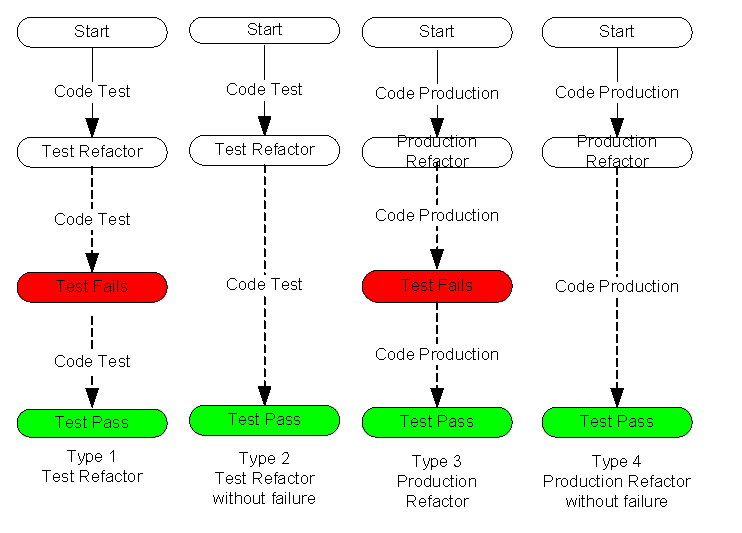
\includegraphics[width=0.8\textwidth]{figs/Refactoring.eps}
  \caption{Refactoring Microprocess Classification}\label{fig:refactoring}
\end{figure} 

\section{Research Statement}
Software engineering is an empirical discipline and best practice is a very
important component in this field. Lacking of good tool support greatly
impacts validity of the research conclusions. My research is to design and
develop a paradigm to facilitate empirical software research on iterative
software processes and best practices effectively by the introduction of
software development stream analysis (SDSA) framwork. I am going to study
how this framework can support Test-Driven Development empirical study in
my thesis work and the weakness of this automation approach. Upon success
this research will power empirical researchers both qualitative evaluation
and quantitative measure of software best practice executions.

\section{Research Methods}

\section{Roadmap}
This thesis work is to evaluate best practice execution in software development 
with development stream. Chapter \ref{chap:relatedwork} is the related
literature work on Hackystat, software process automation, event stream and
Test-Driven Development. The system design structure and implementation details
are described in chapter \ref{chap:implementation}. The framework is tested
against Test-Driven Development with a series of experiments in 
chapter \ref{chap:evaluation}.
\begin{comment}

 as in Figure \ref{fig:EpisodeTree}.
\begin{figure}[htbp] 
  \centering
  \includegraphics[width=0.8\textwidth]{figs/EpisodeTree.eps}
  \caption{Episode Tree}\label{fig:EpisodeTree}
\end{figure} 

Some empirical case studies \cite{George:03}, \cite{Maximilien:03}
reported successes on TDD practice. According to these studies TDD group
passed more black box tests than TLD group and they spent less time on
projects than TLD group. Even though most empirical studies drew positive
conclusion on Test-Driven Development there are still some neutral or
negative reports on TDD. Geras etc. \cite{Geras:04} found that there is
little or no difference in developer productivity in TDD and TLD processes.
Another study \cite{Muller:02} concluded that TDD does not accelerate the
implementation and the resulting programs are not more reliable than TLD.

\section{Validation}
Unlike many other cumbersome software processes such as Spiral model, PSP or
RUP Test-Driven Development is very lightweight. It contains two simple
rules only. In practice TDD is hard to follow compared to other processes
because there is no management involved in the development. In situations
that pair programming is not involved developers are fully responsible for
TDD execution by themselves without monitoring. This weakness will bring
many questions to TDD process. Do developers do Test-Driven Development
when they are told to do so? And if they do how well they do TDD in their
development? Do developers always follow two TDD rules?

In my thesis study I will build a system on top of Hackystat to answer
these questions as well as provide a tool to discipline TDD process.  There
are two goals to pursue in my work. One is to study how the development is
being done, especially how the unit testing is conducted in Test-Driven
Development. Another goal is to study properties of TDD. Will developers
spend more time on development and yield high quality code or not? Will the
test coverage be naturally 100\%?

Scott Ambler's UML diagram (Figure \ref{fig:TDDSteps}) depicts TDD development
iterations.

\begin{figure}[htbp] 
  \centering
  \includegraphics{figs/TDDSteps.eps}
  \caption{The Steps of TDD}\label{fig:TDDSteps}
\end{figure} 

\begin{itemize}
\item The first step is to add a test quickly. Basically it just fails the
  code.
\item Next run your test or test suite to make sure the new test does fail.
\item Make changes to the function code to make test pass. As long as it
  can make test pass you even can fake the implementation, for instance,
  return a constant number.
\item Run your tests again. If it still fails you go ahead to update your
  function code. Once all tests pass you can start over with a new test.
\end{itemize}



 
In the early era of software development there is no software process.
Software systems are developed in a chaotic style and their successes
depended largely on individual's skills and capabilities. Water-fall model
is the first and most popular software development process and it still
exists in many organizations. In water-fall model software development is
divided into stages from requirement analysis to operation and testing is
conducted after project is implemented. Bugs and defects found in testing
will be fed back to the development team or maintenance team. Since bugs
and defects are revealed at the late stage of software development
water-fall model is reluctant to meet customer's requirements and defect
fix. If defects are rooted from design it will be extremely hard to adapt
changes according to water-fall model.

Modern iterative incremental development(IID) was developed to fix this
problem by dividing a large project into many parts.  They are implemented
iteratively. Each iteration can be a mini-waterfall process so that defects
can be fixed and changes can be made very quickly.  Spiral model is the
first process definition to formulate iterative incremental development
practice. Other variations like prototyping, RAD, CleanRoom, Scrum, RUP,
FDD, Extreme Programming are used in many projects successfully.  Latest
development of continuous integration builds system once a day. In these
processes testing is done after some amount of work is finished to improve
project quality.
  
\section{Personal Software Process}
\label{sec:psp}

   Introduce LEAP and Hackystat.

\section{Test-Driven Development}
\label{sec:tdd}

\subsection{Unit Testing}
\label{sec:UnitTest}
Object-oriented technique treats abstract concepts as entities such that
each of them is independent and can exist without relying on other code.
Unit testing was invented to test a component before it is integrated to
interact with other components. Unit testing originates from
pre-object-oriented era and an individual test concentrates on a single
unit of the system rather than on the entire system. At present when we say
unit testing it refers to component testing. In object-oriented world a
component test usually tests an object or class which is the smallest component
of a system. ``In computer programming, a unit test is a method of testing the
correctness of a particular module of source code.'' \cite{UnitTestWiki}

Unit testing is becoming more and more popular in modern software
development.  The de facto unit testing standard, ``xUnit'' framework, is
already ported to more than 30 language support. It makes test automation
be feasible and test cases created with XUnit framework can server as
regression test suite too. Except for verifying correctness of each class
unit testing is also the executing documentation. In recent software
project development unit testing is integrated into development process in
many organizations. Test cases are written by developers who are also
responsible for programs. Even though source code is visible to developers
but unit testing is still thought as black-box testing because it simulates
calls from other components.  

JUnit is the most well-known XUnit framework implementation in software
development and other dialects NUnit, CPPUnit, PyUnit so on and so forth
are created to make writing unit tests be very simple in different
programming languages. JUnit and NUnit also have IDE plug-in supports so
that a unit test case can be exercised by just a single click. For
continuous integration unit test cases can also be batched together to run
as ANT task. Since writing unit tests is not a cumbersome job any more it
is recommended to write unit tests in the development process instead of
allocating extra resource to let quality assurance testers to create unit
tests separately. It improves the effectiveness of testing such that
software systems are in high quality before they are delivered to quality
assurance department or customers if there is no quality assurance process.
Since less time is needed to do quality assurance it will save overall
development time conceptually.


In TDD unit testing is crucial because it drives the implementation and provides
instant feedback of the developing code to the developers. The XUnit
framework family make it easy to write tests and execute tests often in
software development.

\section{Thesis Work}


\section{Road Map}

\end{comment}
\begin{comment}
\label{sec:ResearchObjective}
Test-Driven Development is being accepted by more and more developers and
organizations. On the other side there are still many developers and
researchers resist Test-Driven Development or doubt its effectiveness in
software development. Kent Beck argued that TDD will not increase
development cost but can actually improve productivity as well as software
quality. Ron Jeffries's pithy word ``Clean code that works'' is the goal
of Test-Driven Development.


\section{Extreme Programming(XP) and Test-Driven Development(TDD)}
[How good is unit test? and why TDD]

  
This testing pyramid corresponds to software system development process.
In general a large system is divided into many components to be implemented
independently. Unit testing is created to verify correctness of each
component before it is integrated into the system.
  
Usually unit testing is done by programmers themselves to verify the
correctness or by quality assurance specialists to find errors in the
existing code.  According to the cost model of removing bugs in different
software development stages removing bugs in development phase is the most
cost-effective way.  Because unit testing is good from many aspects Extreme
Programming, an agile software development process, advocates Test-Driven
Development (TDD) as its core component. In TDD unit tests are
incrementally written prior to code implementation \cite{George:03} thus
it drives software specification design in addition to validating and
verifying program correctness. Because of this capability TDD is also
called Test-First Design (TFD). As comparison the old way writing unit
tests after code is ready is called Test-Last Development(TLD).
  
  
  The controversial conclusions can be either from TDD process itself or
  from the poorly executed experiments. There is one thing in common that
  all these studies failed to address how they managed experiments to
  guarantee TDD developers do Test-Driven Development while TLD developers
  do Test-Last Development in their studies. There is no process data
  available to crossly validate process disciplines. The lack of
  fine-grained process data and software metrics makes it impossible to
  conclude whether developers were doing TFD, ad-hoc or TLD in the previous
  experiments; thus, conclusions drawn from these experiments are weakened
  and become questionable. In my thesis I will add in-process metric
  support provided by Hackystat to study how unit tests are created and
  exercised in the development process to regulate software development.
\end{comment}

\begin{comment}  
\section{Testing}
\label{sec:Testing}
Testing is very important to software project success because developers
can not always produce perfect code that works well at the first time. Many
reasons determine that we need testing in software development. First of
all, many software systems deal with large number of states with complex
algorithms, also it is hard and impossible to address all system
requirements at the beginning of software projects development. Developers
always have to deal with new and changing requirements during the
development.  Another important factor is that software projects are
written by developers.  As human beings developers are not good at
repeative programming work without committing mistakes.  Since software
development is error-prone many design and development support tools such
as flowchart, dash board, UML , compilers, debuggers, version control
system, project management software, bug tracking system and software
review etc are brought up to support qualitative software development.
Moreover, there are rare software projects developed and maintained by an
individual programmer nowadays. The ineffective collaboration and
cooperation in the developing team will make software volatile to defects
and bugs too \cite{Pfleeger:01}.  To ensure software quality there are
quality assurance departments in many software institutes and many testing
techniques appeared in the development of software engineering discipline.
From visibility of source code there are white-box testing and black-box
testing. Depending on when testing happens there are unit testing,
regression testing, integration testing, system testing and acceptance
testing which can be done by programmers, quality assurance testers or
customers manually or automatically.

\begin{figure}[ht] 
  \centering
  \includegraphics[width=0.5\textwidth]{figs/TestLayerPyramid.eps}
  \caption{Software Testing Pyramid}\label{fig:TestLayer}
\end{figure} 

In tradition, software testing is thought as quality assurance testers' or
customers' job in water-fall software process model. Even in recent
iterative incremental development (IID) models quality assurance
specialties and customers still play important roles on testing.


\section{Software Processes}
\label{sec:SoftwareProcess}
In the early era of software development there is no software process.
Software systems are developed in a chaotic style and their successes
depended largely on individual's skills and capabilities. Water-fall model
is the first and most popular software development process and it still
exists in many organizations. In water-fall model software development is
divided into stages from requirement analysis to operation and testing is
conducted after project is implemented. Bugs and defects found in testing
will be fed back to the development team or maintenance team. Since bugs
and defects are revealed at the late stage of software development
water-fall model is reluctant to meet customer's requirements and defect
fix. If defects are rooted from design it will be extremely hard to adapt
changes according to water-fall model.

Modern iterative incremental development(IID) was developed to fix this
problem by dividing a large project into many parts.  They are implemented
iteratively. Each iteration can be a mini-waterfall process so that defects
can be fixed and changes can be made very quickly.  Spiral model is the
first process definition to formulate iterative incremental development
practice. Other variations like prototyping, RAD, CleanRoom, Scrum, RUP,
FDD, Extreme Programming are used in many projects successfully.  Latest
development of continuous integration builds system once a day. In these
processes testing is done after some amount of work is finished to improve
project quality.



\section{Extreme Programming}
\label{sec:XP}
Extreme programming (XP) grows very fast recently and many organizations
are using it or considering to adopt it in their developments. Extreme
Programming is also one kind of iterative incremental development (IID)
process.  It begins with collecting ``user stories'', which are brief
description of tasks to be accomplished. Developers can discuss with on-site
customers to make release plan based on user stories. After each release
customer can test the sub system and give feedback to developers quickly.
XP can not only meet customers' changing requirements well but also provide
high quality code because it stresses heavily on unit tests in the
development. Four rules are enforced in extreme programming.

\begin{itemize}
\item All code must have unit tests.
\item All code must pass all unit tests before it can be released.
\item When a bug is found tests are created.
\item Acceptance tests are run often and the score is published.
\end{itemize}

To enact these rules XP projects should be developed in Test-Driven
Development process, in which unit tests are created before code
implementation.  Developers write unit tests based on user stories first
and then generate code to make test pass.
\end{comment}

\chapter{Related Work}
\label{chap:RelatedWork}

\section{Extreme Programming and Test-Driven Development}
\subsection{Extreme Programming}
Extreme Programming (XP) is a light-weight methodology for
small-to-medium-sized teams developing software in the face of vague or
rapidly changing requirements \cite{Beck:00}. It take common-sense
principles and practices to extreme level.
\begin{itemize}
\item If code reviews are good, we'll review code all the time (Pair Programming). 
\item If testing is good, everybody will test all the time (unit testing),
  even the customers (Functional Testing).
\item If design is good, we will make it part of everybody's daily business
  (Refactoring).
\item If simplicity is good, we will always leave the system with the
  simplest design that supports its current functionality (the simplest
  thing that could possibly work).
\item If architecture is important, everybody will work defining and
  refining the architecture all the time (Metaphor).
\item If integration testing is good, then we will integrate and test
  several times a day (Continuous Integration).
\item If short iterations are good, we will make the iteration really,
  really short--seconds and minutes and hours, not weeks and months and
  years (Planning Game).
\end{itemize}

XP is an agile process including 12 practices of: Planning Game, Small
Releases, Metaphor, Simple Design, Testing, Refactoring, Pair Programming,
Collective Code Ownership, Continuous Integration, Forty-hour Week,
On-site Customer and Coding Standards. \cite{Beck:00} As Kent Beck said XP is
not from ground up but many good practices derived from previous software
development. In XP these 12 practices support each other and complement
each other's weakness.  (Figure \ref{fig:XPSupportNetwork} Excerpted from
P70 \cite{Beck:00})
\begin{figure}[ht] 
  \centering
  \includegraphics[width=0.8\textwidth]{figs/XPSupportNetwork.eps}
  \caption{XP Support Network}\label{fig:XPSupportNetwork}
\end{figure} 

A typical XP project starts from planning game. Release plans will be laid
out in the planning game. Each release will vary from several weeks to
several months but not over half a year. Customers or stake holders define
release scope and important or critical business components go first.
Because XP is aiming at building simple but works software the advanced and
not-necessary features will not be considered until demanded. This will
maximize the Return-on-Investment (ROI). Communication, simplicity,
feedback and courage are four values XP will provide. Communications between
customer and developer, coach and developer, inter-developers are
encouraged by XP practices such as on-site customer, metaphor, coding
standard, collective ownership and pair programming directly or indirectly.
Feedback and courage are provided by test-driven development, on-site
customer, pair programming and continuous integration.  Simplicity is the
theme of XP through the entire development.  XP is another kind of
iterative incremental development (IID). The release plan is iterative and
development in each release is iterative too. Iteration in development is
from user story that can last only several days. The task assignment is
done in stand-up meeting. \cite{Beck:00}

Management of XP is through metrics, coaching, tracking and intervention.
It has roles developers, customer, tester, tracker, coach, consultant and
big boss. These roles are responsible for smooth execution and balance
maintenance of all 12 XP practices. Though XP acknowledges that each
practice has its own weakness it is not feasible for a developing team to
tranfer to XP seamlessly. Don Wells \cite{Beck:00} commented that XP
adoption can be iterative:
\begin{enumerate}
\item Pick your worst problem.
\item Solve it in XP way.
\item When it is no longer your worst problem, repeat.
\end{enumerate}

As we already know XP consists of 12 practices. Many of them can exist
independently. Planning game can fit into other IID process. On-site
customer can be available to other process models such as water-fall model.
Among 12 XP practices Pair Programming (PP) and Test-Driven Development
(TDD) often exist independently. They are widely applied and studied by
software developers, educators and researchers.

\subsection{Pair Programming}
Pair programming is an Extreme Programming practice. In pair programming
two programmers sit side-by-side at one computer, continuously
collaborating on same design, algorithm, code or tests. One acts as the
driver who types at computer. Another one acts as the navigator who is
responsible for high-level tasks like over-viewing design strategy,
inspecting code being typed for typos, syntax errors, or defects. Roles in
pair programming are dynamic and they can be exchanged during the
programming session or rotated in different programming sessions. Also the
pairs can be dynamically formed in a developing team. Two people actively
work on the same programming task with continuous collaboration.

Pair programming takes the privilege of code inspection a.k.a. code review
to improve code quality. Even though design or coding errors still can
exist but they will not last long because driver has to explain what he or
she is doing to navigator which provides a chance for both parties to think
it over. It looks like resources are wasted in pair programming because two
developers are invested on tasks that can be done by a solo developer;
however, Laurie Williams's case study concluded that pair programming will
not double development effort. In her study paired programmers are only
15\% slower than two independent individual programmers but produced 15\%
fewer bugs.  The knowing fact is that test and debug cost will be much
higher than initial programming so it will be economically paid off,
especially when some team members have to leave.

In extreme programming pair programming serves multiple purpose. Programs
are written by driver and navigator such that code review is done
simultaneously. The duo continuously communicate for better solution and
everyone inspects other's work. If driver goes the wrong way it can be
adjusted quickly by navigator without committing more mistakes, for
instance, when driver is not creating a test case before implementation
navigator can point it out so that they stay on the right track. Since
driver and navigator are exchanged during development both parties know
code well and own it. In case one programmer has to leave the developing
team risk is minimized because other people can take his or her work
over easily. The other benefit of pair programming is that junior
programmer can be coached and knowledge can spread over in the
team.\cite{PPWiki}

\subsection{Test-Driven Development}
Test-Driven Development is another Extreme Programming practice that has
its own benefits alone like pair programming. It's both the developing
method and design tool in extreme programming. Often it is called
Test-First Design (TFD) or Test-First Programming (TFP) because of its
natures. It has two fundamental rules:
\begin{itemize}
\item Write new code only if an automated test has failed.
\item Eliminate duplication.
\end{itemize}

Development of TDD is iterative. Test and implementation are added
incrementally under these two rules. An iteration can be elaborated as
following \cite{TDDWiki}:

\begin{enumerate}
\item Write the test
\item Write the code
\item Run the automated tests
\item Refactor
\item Repeat
\end{enumerate}

TDD is on the ground of a universally agreed claim that testing is good
to software project success. If it is done perfectly there is no need to
have a coverage tool because system is always 100\% tested. It supports
simplicity since developers only need to write enough code to make test
pass. Refactoring happens at the end of each iteration. Also unit tests can
serve as executing documentation of system so that re-usability is
improved.

In TDD unit tests are supported by XUnit framework. It is brought up by
Kent Beck, Ward Cunningham and Ron Jeffries in 1996 \cite{XP96}. It has the
following structure \cite{Beck:03}:

\begin{enumerate}
\item Invoke test method
\item Invoke setUp first
\item Invoke tearDown afterward
\item Invoke tearDown even if the test method fails
\item Run multiple tests
\item Report collected results
\end{enumerate}

In recent years xUnit has already been ported to more than 30 language
supports such as JUnit for Java, PyUnit for Python, NUnit for C\#.NET,
PHPUnit for PHP, CPPUnit for C++, DUnit for Delphi etc. \cite{XPSoftware}
and it has becoming the de facto standard of unit testing in software
development. With xUnit the unit testing is shifted from quality assurance
specialists or customers to developers.

This framework modulates unit testing onto method level. All public methods
in object-oriented domain are testable with this framework. It moves unit
testing from customer-oriented functional testing to the combination of
developer-oriented unit testing and customer-oriented functional testing.
Once project is brought up for functional testing it is already in high
quality insured by unit testing.

Theoretically speaking it is possible to do TDD perfectly but it is not
feasible in reality. First, developers as human beings are not good at
executing these two rigid rules. Second, there exists many holes such that
it is either not possible to do unit testing to some code or practically
infeasible in some cases. For instance, private methods are not accessible
for test purpose unless developer exposes them; GUI or event-driven methods
are not testable because they need humans intervention to make it happen;
some operations like database accesses are very time consuming such that unit
testing will take long time to run. Because of these limitations developers
would  not be able to follow TDD rules perfectly as Kent Beck wished.

In extreme programming process TDD can be executed better because other
practices can support it as figure \ref{fig:XPSupportNetwork} shows. Pair
programming supports TDD because two brains are better on creating good
unit tests and navigator can inform driver if unit tests are not created
before implementation. Coach can help pairs to design unit testing in case
it is hard or infeasible to do unit testing. Continuous integration can
help developers be aware of some unit tests fail or there is no unit test
to some code.


\section{Test-Driven Development in Practice}
Test-Driven Development is an incremental software development methodology
that stresses on exhausitive unit testing by creating test cases before
code implementation. It's a design and implementation methodology but
testing.  It ends with a rich suite unit test cases and high quality code
as it promises. It appears very often in software development tutorial
workshops
(\cite{OsheroveWorkshop:04,ClarkwareWorkshop:04,BENUGWorkshop:04,AdaptionTddWorkshop,IntustrialLogicTddWorkshop}),
technical reports, journals (\cite{TestDrivenDotComArticles}) and
blogsphere (\cite{TestDrivenDotComWeblogs}). Also many commercial and
open-source supporting tools (\cite{TestDrivenDotComTools}) are developed
in recent years.

\subsection{Characteristics of Test-Driven Development}

\subsubsection{Disciplined Small Steps}
In TDD development is incremental and iterative. Developers only write a
small portion of a unit test, or just one assertation each time, and then
just write enough code to test pass. At the beginnig the test target does
not exist so it cannot pass compilation. For instance, before we create
class Stack for a stack implementation we create a test class called TestStack.

    \begin{verbatim}
    package com.stack;

    import junit.framework.TestCase;

    /**
     * Tests stack operations. 
     */
    public class TestStack extends TestCase {
    }
    \end{verbatim}

To test whether stack can report its emptiness correctly developer adds one
assertation only in the first iteration.

    \begin{verbatim}
      /**
       * Tests empty stack.
       */
      public void testEmptyStack() {
        Stack stack = new Stack();
        assertTrue("Test empty stack", stack.isEmpty());
      }
    \end{verbatim}

It is not runnable because Stack class is not created yet. After creates
dummy implementation or stub of Stack it still cannot be compiled because
isEmpty() is not provided.

    \begin{verbatim}
    package com.stack;

    /**
     * Implements a stack.
     */
    public class Stack {
      /**
       * Constructs a stack.
       */
      public Stack() {
      }
    }
    \end{verbatim}

To make it compile developer goes ahead to add method isEmpty() which just
returns a constant.
    \begin{verbatim}
      /**
       * Whether stack is empty.
       * 
       * @return True if stack is empty.
       */
       public boolean isEmpty() {
         return false;
       }
    \end{verbatim}

Now it compiles but test fails because isEmpty() method simply returns
false. To make test pass developer changes it to return true. Then he/she
can go ahead to add another assertation and test case. As we can see from
above example development pace is really small in TDD. Generally one
iteration or cycle lasts from 30 minutes to 5 minutes. It rarely grows to
10 minutes \cite{GaryPollice:03}. It is totally okay to just add
implementation stub or simply returns a constant value to fake 
implementation (p13 \cite{Beck:03}, p169 \cite{Astels:03}).

\subsubsection{Consistent Refactoring}
Refactoring is an important portion in Test-Driven Development, it the
second TDD rule. By definition, refactoring is a disciplined technique for
restructing an existing body of code, altering its internal structure
without changing its external behavior \cite{Refactoring}. To make it
simple and concise refactoring is to change a program's interal structure
without affecting its external behaviors. In TDD developers need to
consistently do refactoring to support growing test suite without leaving
implementation code badly structured. When we do TDD the first priority is
to get test pass and the next is to remove duplication \cite{Beck:03}.
These two steps fulfil a complete TDD cycle. "Make it run, make it right.''
p24 \cite{Beck:03} Using the above example we can refactor isEmpty()
method to return an instance variable instead of a constant.
    \begin{verbatim}
      private int size = 0;
      /**
       * Whether stack is empty.
       * 
       * @return True if stack is empty.
       */
       public boolean isEmpty() {
         return this.size == 0;
       }
    \end{verbatim}

Now we run TestStack it passes. The duplication can be either on test code
or production code. As long as you get all tests pass you are confident to
do refactoring because unit tests can ensure you will not commit
unrecoverable big mistake.

\subsubsection{Courage, Rapid Feeback and One Ball in the Air at Once}
Kent Beck thinks TDD is a way of managing fear during development
\cite{Beck:03}. Programmers are in fear in software development because the
requirements are not clearly stated, techniques are new, problems are hard
to solve, or there is no enough time to do a thorough design and review.
Fears happen more often to novice programmers but experienced programmers
have fears too because a smallest mistake may break the whole system.
Experience programmers are good at debugging and have better intuition on
finding and solving bugs than novice programmers. In TDD developers ``test
a little, code a little and repeat.''\cite{Beck:03} Test cases guard code
development and provide instant feedback. Since the incremental step is
small it is impossible to commit big mistakes. If test fails it is easy to
fix it too. In software development developers carry the baggage with
requirement, system structure design, algorithm, code efficiency,
readibility and communication with other code etc. According to Martin
Fowler it is like keeping several balls in the air at once (Page 215
\cite{Beck:03}).  In TDD you only keep one ball in the air at once and
concentrate on that ball properly. Developer only needs to make the test
pass without worrying it is a good or bad design in TDD. In refactoring
step developer only worries about what makes a good design. Keeping one
ball only in the air helps doing good job on every aspect.

\subsubsection{Always Working Code}
TDD developers maintain a comprehend unit test suite and all test pass at
the end of each TDD cycle. The developing system is always working to the
designated tasks represented by unit tests. Since all test cases are
created in the domain of xUnit framework they can be integrated together to
do continuous integration. A test bot or agent can be setup to run all
tests everyday or every few hours \cite{ContinuousIntegration}. It works
well especially in team software development or in case it is not feasible
for a developer to run all tests in development in time manner.

\subsection{Benefits of Test-Driven Development}
\subsubsection{100\% Code Coverage}
If it is done perfectly TDD should always yield 100\% code coverage
\cite{Beck:03,Jeffries:00} as figure \ref{fig:TestScores} shows (Excerpted
from page 139 \cite{Jeffries:00}).
 
\begin{figure}[ht] 
  \centering
  \includegraphics[width=0.8\textwidth]{figs/TestScores.eps}
  \caption{Unit Test Scores}\label{fig:TestScores}
\end{figure} 

In practical it is not feasible to maintain 100\% but TDD developers do
yield high code coverage. Boby George and Laurie Williams's study finds
that TDD developers' test cases achieved 98\% method, 92\% statement and
97\% branch coverage \cite{George:02}. The experiment was conducted on a XP
developing team with Pair Programming practice too. Another study conducted
by Matthias M\"uller and Oliver Hagner in University of Karlsruhe found
that TDD developers yielded 74\% median branch coverage \cite{Muller:02}.
It's quite surprising because it is even lower than control group without
doing TDD whose median coverage is 80\%. On the fact that it is impossible
or not necessary to achieve 100\% this test coverage is still low. 

\subsubsection{Regression Test}
One principle of TDD is to create a regression unit test if system breaks.
The test fails first just as a typical TDD iteration. Code isolation is
another TDD principal that reduces coupling between objects. High CBO is
bad in object-oriented programming from modular design and reuse point of
views \cite{CKMetrics}. It's also straight forward the coupling can not be
zero because differant parts have to interact to make the system work. In
TDD developers run all tests regressively to make sure the new change will
not break other parts. Speaking in Java all package should have class
\verb!TestAll!  which assemblies all unit tests in the same package
together. When developer is working she or she just focus on tests in this
small area. XP has another practice called continuous integration to
execute all unit tests in timely manner to check system's consistency. If
the new change breaks system developer will know it in a few hours or a
day. A byproduct of TDD is a very comprehensive and exhaustive test set
that can serve as regression test suite.
 
\subsubsection{Executable Documentation}
In TDD there is no stacked written design documentations instead of
executing design documentation in unit tests. They are system-level
documentation and show how developers intended for the class to be used
\cite{ObjectMentorTDD,Ambler:03}.

\subsubsection{Clear Design}
XP community argues that TDD is not about test but design \cite{North:01}.
There is no big up-front design in XP and TDD but small incremental change.
Design decision is made incrementally by refactoring. Developers do
incremental change to the current code base instead of following design
documentation. Jim Little concluded that this evolutionary design yields
better results than big up-front design \cite{Little:01}. The design
architecture with upfront design generated a five-layer structure for data
persistence which is too complex in practice and the developing team was
completely lost. Intead the evolutionary is easy and effective in
architecture design. Also, TDD developer will not do anything extra except
for passing unit tests. It makes clean code that works \cite{Beck:03} and
is testable.

\subsubsection{High Quality Code}
Probably the most significant benefit of TDD to software development is
high code quality. Generally speaking TDD developers write code with high
coverage and the software created with TDD is more reliable than non-TDD
approach. Matthias M\"uller and Oliver Hagner's experiment in University of
Karlsruhe found that Test First Group (TFG)'s program has higher reliabilty
than controll group's code. In their experiment five TDD developers achieve
reliability over 96\% compared to only one program from the control group
that achieved this\cite{Muller:02}. Using black box test as external
validation TDD pairs passed approximately 18\% more black box tests in case
study conducted by Boby George and Laurie Williams \cite{George:03}.

\subsubsection{Increased Productivity}
TDD is faster test-last and code-N-fix. In TDD, testing is part of the
design process, it doesn't take long time to write a small test
\cite{MemoRandaBlog}. It is faster than test-last because developers need
to spend same amount or more time on creating tests after implementation.
Boby George and Laurie William's study showed that TDD developer spent 16\%
more than controller group but controller group did not primarily write any
worthwhile automated test cases though there were instructed to do so. TDD
code is much more reliable and with high code coverage. Since code is less
buggy it will save a lot time on debugging and maintenace.
\begin{quote}
``I have spent enough time in my career on silly bug-hunting, with TDD those
days are gone. Yes, there are still bugs, but they are fewer and far less
critical'' -- Thomas Eyde \cite{ExtremeJSBlog}
\end{quote}

\subsection{Barriers of Test-Driven Development}
More and more developers turn to TDD and many comercial and free workshops
are provided to evangelize TDD
\cite{TestDrivenDotComWeblogs,TestDrivenDotComArticle}.  Also, many tools
are created to support TDD \cite{TestDrivenDotComTools}. But still, many
developers are reluctant to TDD or even to give it a serious try despite on
the claim that TDD is infective \cite{Beck:03,TestInfected,EichertBlog,MasonBlog}. 
\subsubsection{Testability}
Darach Ennis argued that there are a lot of fallacies blowing around
various engineering organization and among various engineers \cite{Beck:03}. 
\begin{quote}
\begin{itemize}
\item You can't test GUIs automatically (e.g. Swing, CGI, JSP/Servlets/Struts)
\item You can't unit test distributed objects utomatically (e.g., RPC and Messaging style, or CORBA/EJB and JMS)
\item You can't test-first develop your database schema (e.g. JDBC)
\item There is no need to test third party code or code generated by external tools
\item You can't test first develop a language compiler/interpreter from BNF
  to production quality implementation.
\end{itemize}
\end{quote}

Most of these arguments are still valid but some operations are testable
nowadays. JSP and servlets can be tested by HttpUnit\cite{HttpUnit} or
Cactus\cite{Cactus}.  Mock object and Easy Mock can be used to test some
complex operations by providing fake implemention to the real system
\cite{MockObject}.

\subsubsection{Too Much Tests}
TDD is about design. To implement a task or user story developer makes a
list of test cases and maintains it when code grows. When it is empty and
there is no more test case developers can think of, task is done. All code
comes with test and sometimes test code may be larger than production code.
Apparently developers need to spend time on tests which are not thought as
production from customer point of view. XP says that it saves money for
customers on debugging and maintance, which is still not proved yet. A
model about Return on Investment (ROI) of TDD was brought up by Matthias
M\"uller and Frank Padberg shows how TDD can pay off the investment on
test\cite{Muller:03}. So far there is still no case study on cost benefit
analysis on TDD yet.

\subsubsection{Small Steps and Time-Consuming}
In TDD developers make small step each time. There will have many context
swith between test code and production, also many IDE activities. Using
previous isEmpty() method as example.
    \begin{verbatim}
      /**
       * Whether stack is empty.
       * 
       * @return True if stack is empty.
       */
       public boolean isEmpty() {
         return false;
       }
    \end{verbatim}

It is such a trivial thing such that most developers can make it right
without having a failed test. Kent Beck's opinion is that you can write
test that encourages hundreds of lines of code and hours of refactoring but
the tendency of TDD is to have smaller steps over time. Some developers
switched to TDD when old method cannot work, on example is defect removing
in debug.

\subsection{Testing Techniques and Tools}
\subsubsection{XUnit and its Related Tools}
XUnit is the corner stone of TDD. It makes test very simple and test
automation possible. The variation of xUnit includes JUnit for
Java\cite{JUnit}, SUnit for Small Talk\cite{SUnit}, CPPUnit for
C++\cite{CPPUnit}, NUnit for C\#.NET\cite{NUnit}, VBUnit for
VB\cite{VBUnit}, PYUnit for Python\cite{PYUnit} etc.  There are also some
extention for JUnit to test some complex operation, for instance, HttpUnit
for web\cite{HttpUnit}, Cactus for Servlet\cite{Cactus}, and DBUnit for
database\cite{DBUnit}. A new test tool called TestNG is developed to
simplify unit test using annotation and configuration file \cite{TestNG}.

\subsubsection{Mock Object}

\section{Case Studies on Test-Driven Development}
E. Michael Maximilien and Laurie Williams assessed Test-Drive Development
at IBM in the development of a new IBM Retail Store Solutions
version.\cite{Maximilien:03} The initiation of TDD came from the fact that
defect rate of each revisions did not drop in Functional Verification Test
(FVT) though developers have rich domain knowledge. TDD was introduced to
the developing team to alleviate the recurrent quality and testing
problems.  In their study they found defect rate dropped by 50\% in FVT
whereas productivity was not affected.  They believe that the drop of
productivity by TDD was complemented by the adoption of Microsoft Project
Central project management tool. The byproduct of TDD is a substantial
suite of unit tests. They also made test automation be possible and tests
were exercised once a day with the integration support. They also verified
the moral of TDD -- "test-infected'' phrased by Erich Gamma\cite{Beck:03}.
Developers were positive on TDD and intended to continue using it in their
future development.

Boby George and Laurie Williams summarized their findings regarding to
Test-Driven Development in three trial experiments \cite{George:03}.  TDD
approaches yielded superior external code quality measured by a set of
black box tests. TDD developers' code passed 18\% more functional black box
tests than controlled groups' code. Their results also showed that TDD
developers took more time than controlled groups. Additionally controlled
group did not write worthwhile automated test cases, which makes the
comparison on productivity uneven. The projects created by TDD developers
have very high test coverage. The mean method coverage is 98\%, statement
coverage is 92\% and branch coverage is 97\%.

Another case study conducted by Matthias M. M\"uller and Oliver Hagner in
University of Karlstruhe to test development efficiency, resultant code
reliability and program understanding. They found that switching to TDD
does not improve productivity and the code will not be more reliable than
with TDD approach. The only improvement is on code reusability because
tests help developers to use method or interface correctly \cite{Muller:02}.

\section{Hackystat}
Hackystat is an in-process automated metric collection system designed and
built in Collaborative Software Development Laboratory in University of
Hawaii. The attached IDE and ANT build sensors can collect the development
activities including file editing, class creation, method addition and
deletion as well as software metrics like unit test invocations, build
invocations, dynamic object-oriented metrics and other metrics as well.
Using Hackystat rich software metrics can be collected automatically to
study the development process without much work effort involved.

\subsection{Software Metrics}
A software metric is a measure of some property of a piece of software or
its specification \cite{SoftwareMetricWiki:05}. Common software metrics
include source lines of code, object-oriented metrics such as number of
methods in a class, coupling between objects, number of children etc, and
other metrics like function points, bugs per thousand lines of code, code
coverage and so on. Software metrics are widely used in software process to
predict and manage software development. A famous word by Tom Demarco is
that you cannot control what you cannot measure in controlling software
development \cite{SoftwareMetricWiki:05}. Software metrics make software
development process be measurable and process improvement be feasible.  

Koch summarized that there are two sets of objectives of software metrics 
\cite{QPMetricsKoch} :
\begin{itemize}
\item Measures are needed to develop project estimates, to monitor progress
  and performance, and to determine if the software products are of
  acceptable quality.
\item To the software organizations measurement can be used to determine
  overall productivity and quality level, to identify performance trends,
  to better manage software portfolios, to justify investments in new
  technologies, and to help planning and managing the software function. 
\end{itemize}

\subsection{Personal Software Process}
Personal Software Process (PSP) is a manual approach to record personal
software development activities to help project planning and estimation.
It's created and evangelized by Watt Humphrey at Software Engineering
Institute (SEI) in Carneige Mellon University. SEI provides a series of
training courses for developers and educator to grasp it \cite{Humphrey99}.
PSP has four levels range from 0 to 3 and the training course provides 10
programming exercises and five reports. On level 0 developers learn to
record their current practice using time recording log to understand how
time is spent to improve time usage. Other metrics like project size and
defects are measured too on level 0. On level 1 developers will do project
planning and estimation with the metrics data collected to improve
estimation accuracy. Code review and design review are introduced on level
2 to improve personal software quality. Level 3 is called cyclic personal
process. It suggests developers should divide large tasks into small pieces
to develop with PSP as Iterative Incremental Development (IID) advocates.

Many researches and experiments were conducted on PSP. Most of them show
that developers can improve productivity and reduce defect density with PSP
and the estimation accuracy is improved. Some researches reported poor
support for team software development and issue with data collection. Ann
Disney found that data entry is error prone in PSP.

\subsection{Automated Personal Software Process}
PSP helps individual developer to improve personal software process
maturity. To lower data entry overhead and improve PSP data quality.
Carleton A. Moore developed LEAP Toolkit in Collaborative Software
Engineering Laboratory in University of Hawaii. With LEAP Toolkit
developers can record their time and enter data easily. It improves data
accuracy and provides regression analyses that cannot be done manually in
PSP \cite{csdl-99-15}.

\subsection{Hackystat}
Tools like LEAP Toolkits make it fairly easy to record PSP data and conduct
project planning and estimation. In LEAP developers enter PSP data using
clock control and other data entry forms but developers will have to stop
their on-hand work often to input data, which reduces its effectness on
process improvement, project planning and estimation. It is also hard to do
collaboration to support team project development. In 2001 Philip Johnson
etc started Hackystat project to collect development automatically.
Hackystat sensors can be installed in development environments such as
XEmacs, JBuilder, Eclipse and Visual Studio etc to collect software
development data unobtrusively. Hackystat sensors will send out metric data
collected to a centerized data server with SOAP protocol \cite{csdl2-04-05}
in a period-based fashion. Hackystat is extensible so that many kinds of
metrics can be collected except for time, size and defect measurement.
Most development activities such as opening file, editing file, closing
file and refactoring data can be collected by Hackystat sensors. Unit test
case exercises and test coverage can be recorded too by Hackystat. It
supports development collaboration by defining project with common
workspaces\cite{csdl2-04-05}. Initial case studies (\cite{csdl2-03-13},
\cite{csdl2-03-12}) found that Hacksytat has very low overhead for students
and Hackystat analyses are very helpful on student projects. Usage of
Hackystat on extreme programming, high performance computing, project
management and software reviews are being explored in Univeristy of Hawaii
and affiliate organizations.




















\chapter{Implementation}
\label{chap:Implementation}

%%\begin{comment}
\section{Graphic View of Software Testing Process}
Software process is constructed by a series of analysis, design,
development, testing and debugging activities. It starts from requirement
analysis and ends after software products are delivered. Rational Unified
Process (RUP), Personal Software Process (PSP), Team Software Process (TSP)
and Extreme Programming (XP) are some well-defined software processes.
These processes were defined by process pioneers from their best practice
and critical thinkings on their development activities. All processes are
constructed by a set of rules and advices from requirement analyses to
testing. They exist in many kinds of software development organizations and
the rules are enforced by development team leaders or managers. Software
development process is thought as intellectual, non-repeatable and invisible.

In my thesis work I will focus on studying tests in software development,
especially Test-Driven Development to see how tests are being created and
exercised by developers incrementally. A test process view is going to be
implemented to display and analyze how developers create and execute tests
in their development. This tool is called TDPViewer, which stands for Test
Development Process Viewer. With this view support I will be able to
study development process to see whether developers follow a set of
demanded rules.
\section{Process Pattern and Quantification}
Speaking of unit testing execution in software development it could be
either test-first as specified by Test-Driven Development, test-last, or
hybid mode of test-first and test-last. In Hackystat we collect both the
development activities including implementation, compilation, unit testing
and debugging in Eclipse IDE so it is clearly feasible to study how unit
tests are implemented in the development process. Software process rules
can be used to generate development patterns to categorize how developers
do unit testing in the real implementation. One thought here is to design a
rule-based agent to study the development pattern [further research to be
conducted] to do the categorization.
%%\end{comment}





















\chapter{Experiment Design and Claim Evaluation}
\label{chap:Evaluation}
This thesis work introduces software development stream and micro-process
to study software development process. Adoption and learning curves of best
practice in software development impair process development as well as best
practice evaluation. SDSA framework aims at improving both experimental
evaluation and practical execution of best practice in software development
by recognizing micro-process and quantifying best practice execution. 

We will undertake two separated experiments to study correctness and
effectiveness of SDSA in software development best practice evaluation.  In
our study we choose best practice Test-Driven Development as the bechmark
to evaluate our SDSA framework. As a well-known best practice welcomed by
many developers, Test-Driven Development defines two simple rules only such
that experiment subjects can comprehend it easily. Experiment one is best
practice micro-process discovery and validation. The goal of this
experiment is to evaluate how good SDSA can understand development process
and best practice execution. It sets up the benchmark on how system performs
to identify best practice and what kind violations it may detect. In experiment 
two we will use SDSA on a controlled experiment of Test-Driven Development. The
controlled experiment will be the replication of already done experiment on
Test-Driven Development in other organizations. The SDSA-powered experiment
is expected to reveal more detailed information on how test subjects performs
instead vaguely assuming best practices are there. 

\section{Software Development Stream Analysis Framework Validation}
Automatic data collection, development stream contruction, episode
tokenization and micro-process classification are four basic elements of
SDSA framework. This experiment is to test whether it can tell the
difference when developer execute the best practice and when they do not.
Because experiment subjects may or may not have enough skills to write unit
tests, not even to test first we will ask test subjects work on three
problems to build and exercise Test-Driven Development skills. Task 1 is a
simple programming task for us to understand test subject's development
skills, developers should only spend 20 to 40 minutes to finish without
experiment observer's assistance. An optional introduction of unit test
will be provided before subjects work on second experiment. As an
additional requirement we ask all test subject to produce more than 90\%
statement coverage. Experiment assistants will provide technique support to
help test subjects achive high coverage. The coverage is evaluated with
Clover. We will introduce Test-Driven Development before problem 3 and ask
test subjects to work on it following best practice Test-Driven
Development. Similarly as previous experiment we ask for 90\% above
statement coverage too in this experiment.

\subsubsection{Objectives}
Fine tune the development stream construction, episode tokenization and
micro-process classification to measure Test-Driven Development precisely
and differentiate development process quantitatively with SDSA framework.

\subsubsection{Elements of Experiments}
\begin{enumerate}
\item \emph{Subjects} Test subjects are undergraduates who have finished
  one or two 300 level classes already and graduate students. Knowing Java
  and good understanding of Object-Oriented Programming are two basic skills
  required.
\item \emph{Problem Sets} 
  \begin{description} 
  \item Problem 1 is a movie listing management system.  It should be able
    to add a move, delete a movie, modify a move and print out list of all
    movies. Database usage is prohibited for the sake of simplicity and
    user interface is via DOS command line input. It is optional to have
    unit tests. (Approx 20-40 min)
  \item Problem 2 is a stack data structure implementation. Elements in the
    stack are integer objects only. Implemention of stack must be in
    object-oriented style and it test coverage has to be at least 90\%.
    (Approx 20 min)
  \item Problem 3 is a bowling score system. It should tell the correct
    score given a set of bowling throws. We require test subjects write
    programs in Test-Driven Development fashion, and statement coverage
    must reach 90\% at least. In the mean time we want to observe how
    developers conduct Test-Driven Development. Observes will record down
    Test-Driven cycles and violation of Test-Driven Development. We will
    look for an alternative solution to record development process without
    disturbing development work.
  \end{description}
  
\item \emph{Development Tools} Eclipse IDE is the only developement we will
  use in the entire development process. Although Eclipse experience is a
  plus we don't require test subject know Eclipse well to increase our
  chance to recurit approachable test subjects. Development environment
  will be set up by examiners beforehand and we only ask subjects do simple
  tasks only.
\item \emph{Observer and Recorder} It is unsure whethere SDSA framwork can
  canonically reflect development process in the context of Test-Driven
  Development such that we include oberver role in our experiments.
  Observers must know Eclipse well and understand Test-Driven Development
  well. Upon request observers should be able to answer possibly
  sophisicated unit test and Test-Driven Development question. An a
  complement tool we may also monitor and record the development process
  without interfereing test subjects' development process. 
\item \emph{Pre-experiment Survey} Purpose of this experiment is to verify
  SDSA framework implementation so we want diverse test subject population.
  We will include undergraduate, graduate, and possiblely professional
  developers in our experiment. The pre-experiment is informational about
  test subjects.
\item \emph{Post-experiment Survey} Mostly it will be about the test
  subjects' understanding of Test-Driven Development from experiments. 
\end{enumerate}

\subsubsection{Experiment Setup and Procedure}
\subsubsection{Result Analysis}

\section{Evaluation of Test-Driven Development with Assistenance of SDSA framework}
Our motivation to development SDSA framwork is to provide a generic
framework to help best practice practitioners to undertake experiment and
evaluation effectively. Delicate best pracice such as Test-Driven
Development requires high discipline on test subjects, which is hard and
expensive to be managed. The light-weight framework of SDSA powered by
Hackystat will provide in-process development process data. We will replicate
Test-Driven Developments experiments in our study to validate the arguments
contradicted by previous studies.

In the classroom setting we will randomly assign student in the class into
two different groups. They will have the same lecture and teaching
materials.  We require everybody must reach 90\% cover coverage at least.
Group one students has the option to test-last or follow the traditional
water-process. Group 2 students are asked to do Test-Driven Development. In
order to improve the execution effectiveness we ask developer to write a
well-known stack application to improve the understanding of Test-Driven
Development via a tutorial session.

\begin{comment}

This work provides a test development viewer tool to quantatively analyze
Test-Driven Development process using in-process software metrics support.
It can tell whether developer do TDD or not and how unit tests are created
and exercised. In my thesis work I will exam following claims regarding to
TDD with this viewer tool:

\begin{enumerate}
\item 100\% execution of Test-Driven Development is not practical. More or
  less developers will do ad-hoc testing in development, that is to say,
  unit tests are written after implementation code exists.
  
\item TDD helps to yield higher quality code than ad-hoc unit testing and
  TLD. There are significant difference between TDD and TLD.

\item Because of high discipline requirement of TDD, most people will not
  stick to TDD or large portion of their code will not be implemented in TDD
  fashion even though they prefer to it.
\end{enumerate}


To evaluate these claims I propose a series of 5-stage experiments in software
engineering class in spring 2005.

\begin{enumerate}
\item {\bf Skills Building} At beginning of the semester students will
  learn advanced java development skills including Eclipse IDE, JUnit, ANT,
  Hackystat and so forth. They will work on some assignments to practice
  these skills. Hacksytat sensor for Eclipse will be installed as one
  requirement.
  
\item {\bf Project Inition} A semester-long project assignment will be
  given. Students can practice their design, development and unit testing
  skills.

\item {\bf Test-Driven Development} We introduce Test-Driven Development to
  students and ask them to do TDD in their projects. Students can use
  TDDViewer to check their development process.
  
\item {\bf Full-fledged Test-Driven Development} After last round students
  begin mastering TDD. They are required to work on their projects
  following TDD rationals in this iteration.

\item {\bf Post-TDD Adoption} At last step students are free to choose how
  they develop their projects. TDD is not a demand at all.
\end{enumerate}

With this experiment I will be able to test my hypotheses on Test-Driven
Development respectively as following.

\section{Claim 1: Test-Driven Development cannot be done stringently}
Test-Driven Development brings confidence on the code being developed and
also provides other benefits like clear design, robust code, 100\% test
coverage and development effort saving etc. if it can be done perfectly. In
practice this is not applicable even people believe they do TDD very well
in their development process. 

With the educational experiment I can test this by observing how much
portion work is being done in TDD at each iteration. Figure
\ref{fig:TDDTendency} is an example data I may get out of Test-Driven
Development experiment.

\begin{figure}[ht]
  \centering
  \includegraphics[width=0.5\textwidth]{figs/TDDPercentage.eps}
  \caption{TDD Percentage Tendancy}\label{fig:TDDTendency}
\end{figure}
  
This charts shows that more work is done under Test-Driven Development
rationals after students are familar with TDD. In addition to quantatively
telling how much percent work is done in TDD I will also do a survey too.
Appendix A lists the questionnaire to ask students' evaluation and
acceptance to Test-Driven development.

To evaluate this claim I need to supply a pilot implementation which is
done in 100\% TDD. Kent Beck's Cash Exchange example and his footage of
implementation will be used for calibration.

\section{Claim 2: Test-Driven Development yields higher code quality and costs less time}

Assumably Test-Driven Development yields high quality program. In the
experiment if students fail to do TDD well they are likely to produce low
quality code. To evaluate this claim I will collect development active
time, Test-Driven Development active time and code quality evaluation
including number of defects, test coverage and black-box test pass ratio.
Black-box tests are external tests. I will develop a series of black-box
tests to go through all projects to have external validation for code
quality.

Suppose there are 30 black-box tests. Following table contains number of
passed tests to each group. In the table a colum is number of passed tests
under each cateory. To each category average, maximum and minimum values
are listed.

\begin{table}[ht]
\centering
\caption{Number of Passed Tests}
\begin{tabular}{|c|c|c|c|c|} \hline
        &  \textless 50\% & 50-70\% & 70-85\% & 85-100\% \\ \hline
Average & 18 & 22 & 26 & 28 \\ \hline
Minimum & 10 & 15 & 21 & 25 \\ \hline
Maximum & 26 & 25 & 29 & 30 \\ \hline
\end{tabular}
\end{table}


Here block-box test is the proxy for code quality. To course projects,
grading is another proxy to project quality measure. Suppose 60\% out of
100 points will be given to project we may get following distribution.

\begin{table}[ht]
\centering
\caption{Grade v.s. TDD Percentage}
\begin{tabular}{|c|c|c|c|c|} \hline
        &  \textless 50\% & 50-70\% & 70-85\% & 85-100\% \\ \hline
Average & 36 & 44 & 51 & 55 \\ \hline
Minimum & 20 & 33 & 38 & 52 \\ \hline
Maximum & 52 & 51 & 62 & 61  \\ \hline
\end{tabular}
\end{table}

Test coverage will be referred but not a factor to determine code quality
because 100\% code quality can be achieved no matter test is written before
or after code implementation. But I will use test coverage to evaluate
Test-Driven Development because TDD should end with high test coverage even
100\%. Similarly test coverage can be as below.

\begin{table}[ht]
\centering
\caption{Code Coverage v.s. TDD percentage}
\begin{tabular}{|c|c|c|c|c|} \hline
        & \textless 50\% & 50-70\% & 70-85\% & 85-100\% \\ \hline
Average & 70\% & 80\% & 85\% & 90\% \\ \hline
Minimum & 66\% & 75\% & 77\% & 86\% \\ \hline
Maximum & 72\% & 90\% & 91\% & 100\%  \\ \hline
\end{tabular}
\end{table}

I will also look at the development time on test code and production code
to study how much time is spent on them respectively. Theoretically speaking
developers should not spend large amount of time on test code in the development.

\section{Claim 3: Discipline requirement hurdles Test-Driven Development adoption}

It is said developers can get ``test infected'' once they do Test-Driven
Development because of the incrediable confidence and other benefits TDD
brings to them. Once you get infected you will never go back to your old
development habits. It's an interesting issue to address because adoption
is always a problem for new technology. It is even harder for developers to
adopt TDD because it is counter-intuitive. In software development
education students are taught to cut down problems using top-down or
divide-and-conquere analysis skills. Traditionaly unit tests are conducted
by customers or test specialists. Unit testing is not a concern at all
untill Kent Beck came up with Test-Driven Development and xUnit framework.
I hypothesize that people will go back to their old development habits even
though they realize the benefits of Test-Driven Development.

In last iteration of experiment students can choose their development
methods as they want. My expection is that there will be a big drop of
Test-Driven Development percentage as shown in figure
\ref{fig:TDDTendency}. To study why student keep doing or abandon
Test-Driven Development I will conduct a survey to investigate it.


\end{comment}




















\chapter{Time Line}
\label{sec:timelinel}

\begin{table}[ht]
\centering
\caption{Tentative Timeline}
\begin{tabular}{|c|c|} \hline
Task &  Milestone \\ \hline
Pilot Study of TDD and TLD & Jan 7, 05 \\ \hline
Development of TPDViewer & Feb 1, 05 \\ \hline
Form Committee & Feb 1, 05 \\ \hline
First Round TDD Experiment &  Mar 3, 05 \\ \hline
\#1 Survey on TDD Acceptance & Mar 4, 05 \\ \hline
Second Round TDD Experiment & Mar 20, 05 \\ \hline
\#2 Survey on TDD Acceptance & Mar 21, 05 \\ \hline
Third Round TDD Experiment & Apr 15, 05 \\ \hline
\#3 Survey on TDD Adoption & Apr 16, 05 \\ \hline
TDD Study on TDD Adoptors & Aug 8, 05\\ \hline
First Thesis Draft & Oct 10, 05 \\ \hline
Submit thesis to committee  & Nov 15, 04 \\ \hline
Thesis Defense & Dec 3  \\ \hline
\end{tabular}
\end{table}





















\chapter{Conclusion and Discussion}
\label{chap:Conclusion}

\begin{comment}

%hongbing is cool.

To Be Done.

\end{comment}

\appendix
\chapter{Acceptance of Test-Driven Development}


\begin{center}
  Last four digits of your SSN \ldots\ldots\ldots\ldots
\end{center}

\begin{enumerate}
\item I am confident my project is very robust and reliable. \\
(1) Strongly Disagree (2) Disagree (3) Neutral (4) Agree (5) Strongly Agree
\item Test-Driven development helps me to produce simple and working
design.\\
(1) Strongly Disagree (2) Disagree (3) Neutral (4) Agree (5) Strongly Agree
\item I always do refactoring to make my code simple or logic clear. \\
(1) Strongly Disagree (2) Disagree (3) Neutral (4) Agree (5) Strongly Agree
\item Test-Driven Development saves my time on debugging. \\
(1) Strongly Disagree (2) Disagree (3) Neutral (4) Agree (5) Strongly Agree
\item My development time was increased because of Test-Driven Development \\
  (1) Strongly Disagree (2) Disagree (3) Neutral (4) Agree (5) Strongly
  Agree \\ How much percent increase by your estimation? \ldots\ldots  \%
\item I did all my work with Test-Driven Development. \\
(1) Strongly Disagree (2) Disagree (3) Neutral (4) Agree (5) Strongly Agree
\item I will not do Test-Driven Development if it is not required. \\
(1) Strongly Disagree (2) Disagree (3) Neutral (4) Agree (5) Strongly Agree
\item I will recommend Test-Driven Development to my colleagues. \\
(1) Strongly Disagree (2) Disagree (3) Neutral (4) Agree (5) Strongly Agree
\end{enumerate}


\chapter{Test-Driven Development Post-study Questionnaire}

\begin{center}
Last four digits of your SSN \dots\ldots\ldots\ldots
\end{center}

\begin{enumerate}
\item Please specify your development in last session. \\
(1) I did all my work in Test-Driven Development fashion; \\
(2) I did most of my work in Test-Driven Development fashion; \\
(3) Half of my work was done in Test-Driven Development fashion; \\
(4) I occasionally did my work in Test-Driven Development fashion; \\
(5) I did NOT do Test-Driven Development at all. 

\item Compared with last session I feel like my code quality dropped. \\
(1) Strongly Disagree (2) Disagree (3) Neutral (4) Agree (5) Strongly Agree

\item I do Test-Driven Development only when I am NOT confident with my program. \\
  (1) Strongly Disagree (2) Disagree (3) Neutral (4) Agree (5) Strongly
  Agree (6) N/A
  
\item I think writing tests before code implementation is NOT a natural way to 
develop software  \\
  (1) Strongly Disagree (2) Disagree (3) Neutral (4) Agree (5) Strongly
  Agree

\item I think unit test is NOT product. We should leave it to test specialists.  \\
(1) Strongly Disagree (2) Disagree (3) Neutral (4) Agree (5) Strongly Agree

\item I wanted to do 100\% Test-Driven Development but I do NOT know how to 
write tests for some applications. \\
(1) Strongly Disagree (2) Disagree (3) Neutral (4) Agree (5) Strongly Agree
(6) N/A

\item What are the drawbacks of Test-Driven Development from your view 
that prevent it from being widely used? \\
\ldots\dotfill\ldots \\
\ldots\dotfill\ldots

\item If you still do Test-Driven Development and plan to use it in
your future software development please specifye reasons.\\
\ldots\dotfill\ldots \\
\ldots\dotfill\ldots

\end{enumerate}










\bibliography{/export/home/csdl/bib/tdd,/export/home/csdl/bib/csdl-trs,/export/home/csdl/bib/psp}
\bibliographystyle{plain}

\end{document}



















